\chapter{定积分}

\section{定积分概念}

\subsection{问题提出}

不定积分和定积分是积分学中的两大基本问题. 求不定积分是求导数的逆运算, 定积分则是某种特殊和式的极限, 它们之间既有区别又有联系. 现在先从两个例子来看定积分概念是怎样提出来的.

1. 曲边梯形的面积 设 \(f\) 为闭区间 \(\left\lbrack  {a,b}\right\rbrack\) 上的连续函数,且 \(f\left( x\right)  \geq  0\) . 由曲线 \(y =\)  \(f\left( x\right)\) ,直线 \(x = a,x = b\) 以及 \(x\) 轴所围成的平面图形 (图 9-1),称为曲边梯形. 下面讨论曲边梯形的面积 (这是求任何曲线边界图形面积的基础).

在初等数学里, 圆面积是用一系列边数无限增多的内接 (或外切) 正多边形面积的极限来定义的. 现在我们仍用类似的办法来定义曲边梯形的面积.

在区间 \(\left\lbrack  {a,b}\right\rbrack\) 上任取 \(n - 1\) 个分点,它们依次为
\[
a = {x}_{0} < {x}_{1} < {x}_{2} < \cdots  < {x}_{n - 1} < {x}_{n} = b,
\]
这些点把 \(\left\lbrack  {a,b}\right\rbrack\) 分割成 \(n\) 个小区间 \(\left\lbrack  {{x}_{i - 1},{x}_{i}}\right\rbrack  ,i = 1,2,\cdots ,n\) . 再用直线 \(x = {x}_{i}\) , \(i = 1,2,\cdots ,n - 1\) 把曲边梯形分割成 \(n\) 个小曲边梯形 (图 9-2).

\begin{figure}
	\centering
	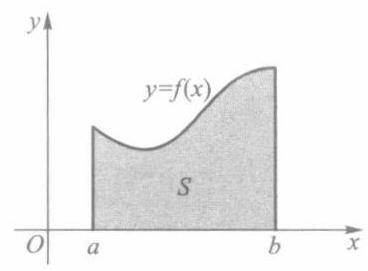
\includegraphics[width=.3\textwidth]{images/P053.jpg}
	\caption{图 $9-1$}
	\label{fig:P053}
\end{figure}

\begin{figure}
	\centering
	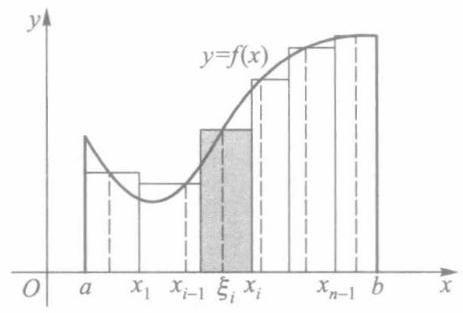
\includegraphics[width=.3\textwidth]{images/P054.jpg}
	\caption{图 $9-2$}
	\label{fig:P054}
\end{figure}

在每个小区间 \(\left\lbrack  {{x}_{i - 1},{x}_{i}}\right\rbrack\) 上任取一点 \({\xi }_{i}\) ,作以 \(f\left( {\xi }_{i}\right)\) 为高, \(\left\lbrack  {{x}_{i - 1},{x}_{i}}\right\rbrack\) 为底的小矩形. 当分割 \(\left\lbrack  {a,b}\right\rbrack\) 的分点较多,又分割得较细密时,由于 \(f\) 为连续函数,它在每个小区间上的值变化不大,从而可用这些小矩形的面积近似替代相应小曲边梯形的面积. 于是,这 \(n\) 个小矩形面积之和就可作为该曲边梯形面积 \(S\) 的近似值,即
\[
S \approx  \mathop{\sum }\limits_{{i = 1}}^{n}f\left( {\xi }_{i}\right) \Delta {x}_{i}\;\left( {\Delta {x}_{i} = {x}_{i} - {x}_{i - 1}}\right) . \tag{1}
\]
注意到 (1) 式右边的和式既依赖于对区间 \(\left\lbrack  {a,b}\right\rbrack\) 的分割,又与所有中间点 \({\xi }_{i}\left( {i = 1,2,\cdots ,n}\right)\) 的取法有关. 当分点无限增多,且对 \(\left\lbrack  {a,b}\right\rbrack\) 无限细分时,如果此和式与某一常数无限接近,而且与分点 \({x}_{i}\) 和中间点 \({\xi }_{i}\) 的选取无关,则自然地,我们把此常数定义为该曲边梯形的面积 \(S\) .

2. 变力所做的功 设质点受力 \(F\) 的作用沿 \(x\) 轴由点 \(a\) 移动到点 \(b\) ,并设 \(F\) 处处平行于 \(x\) 轴 (图 9-3). 如果 \(F\) 为常力,则它对质点所做的功为 \(W = F\left( {b - a}\right)\) . 现在的问题是, \(F\) 为变力,它连续依赖于质点所在位置的坐标 \(x\) ,即 \(F = F\left( x\right) ,x \in  \left\lbrack  {a,b}\right\rbrack\) 为一连续函数,此时 \(F\) 对质点所做的功 \(W\) 又该如何计算?

\begin{figure}
	\centering
	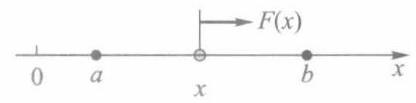
\includegraphics[width=.3\textwidth]{images/P055.jpg}
	\caption{图 $9-3$}
	\label{fig:P055}
\end{figure}

由假设 \(F\left( x\right)\) 为一连续函数,故在很小的一段位移区间上 \(F\left( x\right)\) 可以近似地看作一常量. 类似于求曲边梯形面积那样,把 \(\left\lbrack  {a,b}\right\rbrack\) 细分为 \(n\) 个小区间 \(\left\lbrack  {{x}_{i - 1},{x}_{i}}\right\rbrack  ,\Delta {x}_{i} = {x}_{i} - {x}_{i - 1},i\)  \(= 1,2,\cdots ,n\) ; 并在每个小区间上任取一点 \({\xi }_{i}\) ,就有
\[
F\left( x\right)  \approx  F\left( {\xi }_{i}\right) ,x \in  \left\lbrack  {{x}_{i - 1},{x}_{i}}\right\rbrack  ,i = 1,2,\cdots ,n.
\]
于是,质点从 \({x}_{i - 1}\) 位移到 \({x}_{i}\) 时,力 \(F\) 所做的功就近似等于 \(F\left( {\xi }_{i}\right) \Delta {x}_{i}\) ,从而
\[
W \approx  \mathop{\sum }\limits_{{i = 1}}^{n}F\left( {\xi }_{i}\right) \Delta {x}_{i}. \tag{2}
\]
同样地,对 \(\left\lbrack  {a,b}\right\rbrack\) 作无限细分时,若 (2) 式右边的和式与某一常数无限接近,则我们把此常数定义为该变力所做的功 \(W\) .

上面两个例子, 一个是计算曲边梯形面积的几何问题, 另一个是求变力做功的力学问题, 它们最终都归结为一个特定形式的和式逼近. 在科学技术中还有许多同样类型的数学问题,解决这类问题的思想方法概括说来就是“分割,近似求和,取极限”. 这就是产生定积分概念的背景.

\subsection{定积分的定义}

%定义  1
\begin{definition}{}{def:}

\end{definition}
设闭区间 \(\left\lbrack  {a,b}\right\rbrack\) 上有 \(n - 1\) 个点,依次为
\[
a = {x}_{0} < {x}_{1} < {x}_{2} < \cdots  < {x}_{n - 1} < {x}_{n} = b,
\]
它们把 \(\left\lbrack  {a,b}\right\rbrack\) 分成 \(n\) 个小区间 \({\Delta }_{i} = \left\lbrack  {{x}_{i - 1},{x}_{i}}\right\rbrack  ,i = 1,2,\cdots ,n\) . 这些分点或这些闭子区间构成对 \(\left\lbrack  {a,b}\right\rbrack\) 的一个分割,记为
\[
T = \left\{  {{x}_{0},{x}_{1},\cdots ,{x}_{n}}\right\}  \text{ 或 }\left\{  {{\Delta }_{1},{\Delta }_{2},\cdots ,{\Delta }_{n}}\right\}  \text{ . }
\]
小区间 \({\Delta }_{i}\) 的长度为 \(\Delta {x}_{i} = {x}_{i} - {x}_{i - 1}\) ,并记
\[
\parallel T\parallel  = \mathop{\max }\limits_{{1 \leq  i \leq  n}}\left\{  {\Delta {x}_{i}}\right\}  ,
\]
称为分割 \(T\) 的模.

%注
\begin{remark}

\end{remark}
由于 \(\Delta {x}_{i} \leq  \parallel T\parallel ,i = 1,2,\cdots ,n\) ,因此 \(\parallel T\parallel\) 可用来反映 \(\left\lbrack  {a,b}\right\rbrack\) 被分割的细密程度. 另外,分割 \(T\) 一旦给出, \(\parallel T\parallel\) 就随之而确定; 但是,具有同一细度 \(\parallel T\parallel\) 的分割 \(T\) 却有无限多个.

%定义  2
\begin{definition}{}{def:}

\end{definition}
设 \(f\) 是定义在 \(\left\lbrack  {a,b}\right\rbrack\) 上的一个函数. 对于 \(\left\lbrack  {a,b}\right\rbrack\) 的一个分割 \(T = \left\{  {\Delta }_{1}\right.\) , \(\left. {{\Delta }_{2},\cdots ,{\Delta }_{n}}\right\}\) ,任取点 \({\xi }_{i} \in  {\Delta }_{i},i = 1,2,\cdots ,n\) ,并作和式
\[
\mathop{\sum }\limits_{{i = 1}}^{n}f\left( {\xi }_{i}\right) \Delta {x}_{i}
\]
称此和式为函数 \(f\) 在 \(\left\lbrack  {a,b}\right\rbrack\) 上的一个积分和,也称黎曼和.

显然,积分和既与分割 \(T\) 有关,又与所选取的点集 \(\left\{  {\xi }_{i}\right\}\) 有关.

%定义  3
\begin{definition}{}{def:}

\end{definition}
设 \(f\) 是定义在 \(\left\lbrack  {a,b}\right\rbrack\) 上的一个函数, \(J\) 是一个确定的实数. 若对任给的正数 \(\varepsilon\) ,总存在某一正数 \(\delta\) ,使得对 \(\left\lbrack  {a,b}\right\rbrack\) 的任何分割 \(T\) ,以及在其上任意选取的点集 \(\left\{  {\xi }_{i}\right\}\) ,只要 \(\parallel T\parallel  < \delta\) ,就有
\[
\left| {\mathop{\sum }\limits_{{i = 1}}^{n}f\left( {\xi }_{i}\right) \Delta {x}_{i} - J}\right|  < \varepsilon ,
\]
则称函数 \(f\) 在区间 \(\left\lbrack  {a,b}\right\rbrack\) 上可积或黎曼可积; 数 \(J\) 称为 \(f\) 在 \(\left\lbrack  {a,b}\right\rbrack\) 上的定积分或黎曼积分, 记作
\[
J = {\int }_{a}^{b}f\left( x\right) \mathrm{d}x. \tag{3}
\]
其中 \(f\) 称为被积函数, \(x\) 称为积分变量, \(\left\lbrack  {a,b}\right\rbrack\) 称为积分区间, \(a,b\) 分别称为这个定积分的下限和上限.

以上定义 1 至定义 3 是定积分抽象概念的完整叙述. 下面是与定积分概念有关的几点补充注释.

%注
\begin{remark}

\end{remark}
1 把定积分定义的 \(\varepsilon  - \delta\) 说法和函数极限的 \(\varepsilon  - \delta\) 说法相对照,便会发现两者有相似的陈述方式, 因此我们也常用极限符号来表达定积分, 即把它写作
\[
J = \mathop{\lim }\limits_{{\parallel T\parallel  \rightarrow  0}}\mathop{\sum }\limits_{{i = 1}}^{n}f\left( {\xi }_{i}\right) \Delta {x}_{i} = {\int }_{a}^{b}f\left( x\right) \mathrm{d}x. \tag{4}
\]
然而,积分和的极限与函数的极限之间其实有着很大的区别: 在函数极限 \(\mathop{\lim }\limits_{{x \rightarrow  a}}f\left( x\right)\) 中, 对每一个极限变量 \(x\) 来说, \(f\left( x\right)\) 的值是唯一确定的; 而对于积分和的极限而言,每一个 \(\parallel T\parallel\) 并不唯一对应积分和的一个值. 这使得积分和的极限要比通常的函数极限复杂得多.

%注
\begin{remark}

\end{remark}
2 可积性是函数的又一分析性质. 稍后 (定理 9.3) 就会知道连续函数是可积的, 于是本节开头两个实例都可用定积分记号来表示:

1) 连续曲线 \(y = f\left( x\right)  \geq  0\) 在 \(\left\lbrack  {a,b}\right\rbrack\) 上形成的曲边梯形面积为 \(S = {\int }_{a}^{b}f\left( x\right) \mathrm{d}x\) ;

2) 在连续变力 \(F\left( x\right)\) 作用下,质点从 \(a\) 位移到 \(b\) 所做的功为 \(W = {\int }_{a}^{b}F\left( x\right) \mathrm{d}x\) .

%注
\begin{remark}

\end{remark}
3 (定积分的几何意义) 由上述 1) 看到,对于 \(\left\lbrack  {a,b}\right\rbrack\) 上的连续函数 \(f\) ,当 \(f\left( x\right)  \geq  0,x \in  \left\lbrack  {a,b}\right\rbrack\) 时,定积分 (3) 的几何意义就是该曲边梯形的面积; 当 \(f\left( x\right)  \leq  0,x \in\)  \(\left\lbrack  {a,b}\right\rbrack\) 时, \(J =  - {\int }_{a}^{b}\left\lbrack  {-f\left( x\right) }\right\rbrack  \mathrm{d}x\) 是位于 \(x\) 轴下方的曲边梯形面积的相反数,不妨称之为 “负面积”; 对于一般非定号的 \(f\left( x\right)\) 而言 (图 9-4),定积分 \(J\) 的值则是曲线 \(y = f\left( x\right)\) 在 \(x\) 轴上方部分所有曲边梯形的正面积与下方部分所有曲边梯形的负面积的代数和.

%注
\begin{remark}

\end{remark}
4 定积分作为积分和的极限,它的值只与被积函数 \(f\) 和积分区间 \(\left\lbrack  {a,b}\right\rbrack\) 有关, 而与积分变量所用的符号无关, 即
\[
{\int }_{a}^{b}f\left( x\right) \mathrm{d}x = {\int }_{a}^{b}f\left( t\right) \mathrm{d}t = {\int }_{a}^{b}f\left( \theta \right) \mathrm{d}\theta  = \cdots .
\]
%例 1
\begin{example}

\end{example}
求在区间 \(\left\lbrack  {0,1}\right\rbrack\) 上,以抛物线 \(y = {x}^{2}\) 为曲边的曲边三角形的面积 (图 9-5).

\begin{figure}
	\centering
	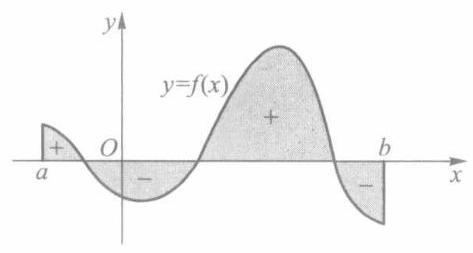
\includegraphics[width=.3\textwidth]{images/P056.jpg}
	\caption{图 $9-4$}
	\label{fig:P056}
\end{figure}

\begin{figure}
	\centering
	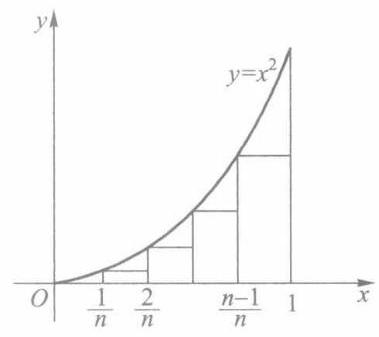
\includegraphics[width=.3\textwidth]{images/P057.jpg}
	\caption{图 $9-5$}
	\label{fig:P057}
\end{figure}

%解
\begin{solution}

\end{solution}
由注 3,因 \(y = {x}^{2}\) 在 \(\left\lbrack  {0,1}\right\rbrack\) 上连续,故所求面积为
\[
S = {\int }_{0}^{1}{x}^{2}\mathrm{\;d}x = \mathop{\lim }\limits_{{\parallel T\parallel  \rightarrow  0}}\mathop{\sum }\limits_{{i = 1}}^{n}{\xi }_{i}^{2}\Delta {x}_{i}.
\]
为求得此极限,在定积分存在的前提下,允许选择某种特殊的分割 \(T\) 和特殊的点集 \(\left\{  {\xi }_{i}\right\}\) . 在此只需取等分分割
\[
T = \left\{  {0,\frac{1}{n},\frac{2}{n},\cdots ,\frac{n - 1}{n},1}\right\}  ,\parallel T\parallel  = \frac{1}{n};
\]
并取 \({\xi }_{i} = \frac{i - 1}{n} \in  \left\lbrack  {\frac{i - 1}{n},\frac{i}{n}}\right\rbrack  ,i = 1,2,\cdots ,n\) . 则有
\[
S = \mathop{\lim }\limits_{{n \rightarrow  \infty }}\mathop{\sum }\limits_{{i = 1}}^{n}{\left( \frac{i - 1}{n}\right) }^{2} \cdot  \frac{1}{n} = \mathop{\lim }\limits_{{n \rightarrow  \infty }}\frac{1}{{n}^{3}}\mathop{\sum }\limits_{{i = 1}}^{n}{\left( i - 1\right) }^{2}
\]
\[
= \mathop{\lim }\limits_{{n \rightarrow  \infty }}\frac{\left( {n - 1}\right) n\left( {{2n} - 1}\right) }{6{n}^{3}} = \frac{1}{3}.
\]
\subsection{习题 9.1}

1. 按定积分定义证明: \({\int }_{a}^{b}k\mathrm{\;d}x = k\left( {b - a}\right)\) .

2. 通过对积分区间作等分分割,并取适当的点集 \(\left\{  {\xi }_{i}\right\}\) ,把定积分看作是对应的积分和的极限,来计算下列定积分:

(1) \({\int }_{0}^{1}{x}^{3}\mathrm{\;d}x\) ; (提示: \(\mathop{\sum }\limits_{{i = 1}}^{n}{i}^{3} = \frac{1}{4}{n}^{2}{\left( n + 1\right) }^{2}\) .

(2) \({\int }_{0}^{1}{\mathrm{e}}^{x}\mathrm{\;d}x\) ； (3) \({\int }_{a}^{b}{\mathrm{e}}^{x}\mathrm{\;d}x\) ;

(4) \({\int }_{a}^{b}\frac{\mathrm{d}x}{{x}^{2}}\left( {0 < a < b}\right)\) .(提示:取 \({\xi }_{i} = \sqrt{{x}_{i - 1}{x}_{i}}\) .)

\section{牛顿一莱布尼茨公式}

从上节例题和习题看到, 通过求积分和的极限来计算定积分一般是很困难的. 下面要介绍的牛顿一莱布尼茨公式不仅为定积分计算提供了一个有效的方法, 而且在理论上把定积分与不定积分联系了起来.

%定理 9.1
\begin{theorem}{}{the:}

\end{theorem}
 若函数 \(f\) 在 \(\left\lbrack  {a,b}\right\rbrack\) 上连续,且存在原函数 \(F\) ,即 \({F}^{\prime }\left( x\right)  = f\left( x\right) ,x \in  \left\lbrack  {a,b}\right\rbrack\) , 则 \(f\) 在 \(\left\lbrack  {a,b}\right\rbrack\) 上可积,且
\[
{\int }_{a}^{b}f\left( x\right) \mathrm{d}x = F\left( b\right)  - F\left( a\right) . \tag{1}
\]
上式称为牛顿一莱布尼茨公式, 它也常写成
\[
{\int }_{a}^{b}f\left( x\right) \mathrm{d}x = {\left. F\left( x\right) \right| }_{a}^{b}.
\]
%证
\begin{proof}

\end{proof}
由定积分定义,任给 \(\varepsilon  > 0\) ,要证存在 \(\delta  > 0\) ,当 \(\parallel T\parallel  < \delta\) 时,有 \(\left| {\mathop{\sum }\limits_{{i = 1}}^{n}f\left( {\xi }_{i}\right) \Delta {x}_{i} - \left\lbrack  {F\left( b\right)  - F\left( a\right) }\right\rbrack  }\right|  < \varepsilon\) . 下面证明满足如此要求的 \(\delta\) 确实是存在的.

事实上,对于 \(\left\lbrack  {a,b}\right\rbrack\) 的任一分割 \(T = \left\{  {a = {x}_{0},{x}_{1},\cdots ,{x}_{n} = b}\right\}\) ,在每个小区间 \(\left\lbrack  {{x}_{i - 1},{x}_{i}}\right\rbrack\) 上对 \(F\left( x\right)\) 使用拉格朗日中值定理,则分别存在 \({\eta }_{i} \in  \left( {{x}_{i - 1},{x}_{i}}\right) ,i = 1,2,\cdots ,n\) ,使得
\[
F\left( b\right)  - F\left( a\right)  = \mathop{\sum }\limits_{{i = 1}}^{n}\left\lbrack  {F\left( {x}_{i}\right)  - F\left( {x}_{i - 1}\right) }\right\rbrack
\]
\[
= \mathop{\sum }\limits_{{i = 1}}^{n}{F}^{\prime }\left( {\eta }_{i}\right) \Delta {x}_{i} = \mathop{\sum }\limits_{{i = 1}}^{n}f\left( {\eta }_{i}\right) \Delta {x}_{i}. \tag{2}
\]
因为 \(f\) 在 \(\left\lbrack  {a,b}\right\rbrack\) 上连续,从而一致连续,所以对上述 \(\varepsilon  > 0\) ,存在 \(\delta  > 0\) ,当 \({x}^{\prime }\) , \({x}^{\prime \prime } \in  \left\lbrack  {a,b}\right\rbrack\) 且 \(\left| {{x}^{\prime } - {x}^{\prime \prime }}\right|  < \delta\) 时,有
\[
\left| {f\left( {x}^{\prime }\right)  - f\left( {x}^{\prime \prime }\right) }\right|  < \frac{\varepsilon }{b - a}.
\]
于是,当 \(\Delta {x}_{i} \leq  \parallel T\parallel  < \delta\) 时,任取 \({\xi }_{i} \in  \left\lbrack  {{x}_{i - 1},{x}_{i}}\right\rbrack\) ,便有 \(\left| {{\xi }_{i} - {\eta }_{i}}\right|  < \delta\) ,这就证得
\[
\left| {\mathop{\sum }\limits_{{i = 1}}^{n}f\left( {\xi }_{i}\right) \Delta {x}_{i} - \left\lbrack  {F\left( b\right)  - F\left( a\right) }\right\rbrack  }\right|
\]
\[
= \left| {\mathop{\sum }\limits_{{i = 1}}^{n}\left\lbrack  {f\left( {\xi }_{i}\right)  - f\left( {\eta }_{i}\right) }\right\rbrack  \Delta {x}_{i}}\right|
\]
\[
\leq  \mathop{\sum }\limits_{{i = 1}}^{n}\left| {f\left( {\xi }_{i}\right)  - f\left( {\eta }_{i}\right) }\right| \Delta {x}_{i}
\]
\[
< \frac{\varepsilon }{b - a} \cdot  \mathop{\sum }\limits_{{i = 1}}^{n}\Delta {x}_{i} = \varepsilon .
\]
所以 \(f\) 在 \(\left\lbrack  {a,b}\right\rbrack\) 上可积,且有公式 (1) 成立.

%注
\begin{remark}

\end{remark}
1 在应用牛顿一莱布尼茨公式时, \(F\left( x\right)\) 可由积分法求得.

%注
\begin{remark}

\end{remark}
2 定理条件尚可适当减弱, 例如:

1) 对 \(F\) 的要求可减弱为: 在 \(\left\lbrack  {a,b}\right\rbrack\) 上连续,在(a, b)上可导,且 \({F}^{\prime }\left( x\right)  =\)  \(f\left( x\right) ,x \in  \left( {a,b}\right)\) . 这不影响定理的证明.

2) 对 \(f\) 的要求可减弱为: 在 \(\left\lbrack  {a,b}\right\rbrack\) 上可积 (不一定连续). 这时 (2) 式仍成立,且由 \(f\) 在 \(\left\lbrack  {a,b}\right\rbrack\) 上可积,(2)式右边当 \(\parallel T\parallel  \rightarrow  0\) 时的极限就是 \({\int }_{a}^{b}f\left( x\right) \mathrm{d}x\) ,而左边恒为一常数. (更一般的情形参见本节习题第 3 题.)

%注
\begin{remark}

\end{remark}
3 至 §5 证得连续函数必有原函数之后,本定理的条件中对 \(F\) 的假设便是多余的了.

%例 1
\begin{example}

\end{example}
利用牛顿一莱布尼茨公式计算下列定积分:

(1) \({\int }_{a}^{b}{x}^{n}\mathrm{\;d}x\left( {n\text{ 为正整数 }}\right)\) ； 

(2) \({\int }_{a}^{b}{\mathrm{e}}^{x}\mathrm{\;d}x\) ;

(3) \({\int }_{a}^{b}\frac{\mathrm{d}x}{{x}^{2}}\left( {0 < a < b}\right)\) ;

(4) \({\int }_{0}^{\pi }\sin x\mathrm{\;d}x\) ;

(5) \({\int }_{0}^{2}x\sqrt{4 - {x}^{2}}\mathrm{\;d}x\) .

%解
\begin{solution}

\end{solution}
其中 (1) 一 (3) 即为 §1 中的例题和习题,现在用牛顿一莱布尼茨公式来计算就十分方便:

(1) \({\int }_{a}^{b}{x}^{n}\mathrm{\;d}x = {\left. \frac{{x}^{n + 1}}{n + 1}\right| }_{a}^{b} = \frac{1}{n + 1}\left( {{b}^{n + 1} - {a}^{n + 1}}\right)\) ;

(2) \({\int }_{a}^{b}{\mathrm{e}}^{x}\mathrm{\;d}x = {\left. {\mathrm{e}}^{x}\right| }_{a}^{b} = {\mathrm{e}}^{b} - {\mathrm{e}}^{a}\) ;

(3) \({\int }_{a}^{b}\frac{\mathrm{d}x}{{x}^{2}} =  - {\left. \frac{1}{x}\right| }_{a}^{b} = \frac{1}{a} - \frac{1}{b}\) ;

(4) \({\int }_{0}^{\pi }\sin x\mathrm{\;d}x =  - {\left. \cos x\right| }_{0}^{\pi } = 2\) .

(这里的 (4) 是图 9-6 所示正弦曲线一拱下的面积, 其余各题也可作此联想.)

(5)先用不定积分法求出 \(f\left( x\right)  = x\sqrt{4 - {x}^{2}}\) 的任一原函数, 然后完成定积分计算:
\[
\int x\sqrt{4 - {x}^{2}}\mathrm{\;d}x =  - \frac{1}{2}\int \sqrt{4 - {x}^{2}}\mathrm{\;d}\left( {4 - {x}^{2}}\right)
\]
\[
=  - \frac{1}{3}\sqrt{{\left( 4 - {x}^{2}\right) }^{3}} + C,
\]
\[
{\int }_{0}^{2}x\sqrt{4 - {x}^{2}}\mathrm{\;d}x =  - {\left. \frac{1}{3}\sqrt{{\left( 4 - {x}^{2}\right) }^{3}}\right| }_{0}^{2} = \frac{8}{3}.
\]
\begin{figure}
	\centering
	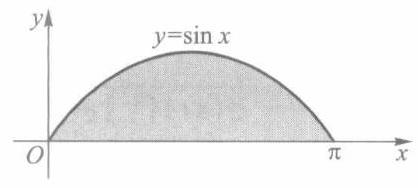
\includegraphics[width=.3\textwidth]{images/P058.jpg}
	\caption{图 $9-6$}
	\label{fig:P058}
\end{figure}

%例 2
\begin{example}

\end{example}
利用定积分求极限
\[
\mathop{\lim }\limits_{{n \rightarrow  \infty }}\left( {\frac{1}{n + 1} + \frac{1}{n + 2} + \cdots  + \frac{1}{2n}}\right)  = J.
\]
%解
\begin{solution}

\end{solution}
把此极限式化为某个积分和的极限式, 并转化为计算定积分. 为此作如下变形:
\[
J = \mathop{\lim }\limits_{{n \rightarrow  \infty }}\mathop{\sum }\limits_{{i = 1}}^{n}\frac{1}{1 + \frac{i}{n}} \cdot  \frac{1}{n}.
\]
不难看出,其中的和式是函数 \(f\left( x\right)  = \frac{1}{1 + x}\) 在区间 \(\left\lbrack  {0,1}\right\rbrack\) 上的一个积分和 (这里所取的是等分分割, \(\Delta {x}_{i} = \frac{1}{n},{\xi }_{i} = \frac{i}{n} \in  \left\lbrack  {\frac{i - 1}{n},\frac{i}{n}}\right\rbrack  ,i = 1,2,\cdots ,n)\) . 所以
\[
J = {\int }_{0}^{1}\frac{\mathrm{d}x}{1 + x} = {\left. \ln \left( 1 + x\right) \right| }_{0}^{1} = \ln 2.
\]
当然,也可把 \(J\) 看作 \(f\left( x\right)  = \frac{1}{x}\) 在 \(\left\lbrack  {1,2}\right\rbrack\) 上的定积分,同样有
\[
J = {\int }_{1}^{2}\frac{\mathrm{d}x}{x} = {\int }_{2}^{3}\frac{\mathrm{d}x}{x - 1} = \cdots  = \ln 2.
\]
\subsection{习题 9.2}

1. 计算下列定积分:

(1) \({\int }_{0}^{1}\left( {{2x} + 3}\right) \mathrm{d}x\) ;

(2) \({\int }_{0}^{1}\frac{1 - {x}^{2}}{1 + {x}^{2}}\mathrm{\;d}x\) ；

(3) \({\int }_{\mathrm{e}}^{{\mathrm{e}}^{2}}\frac{\mathrm{d}x}{x\ln x}\) ;

(4) \({\int }_{0}^{1}\frac{{\mathrm{e}}^{x} - {\mathrm{e}}^{-x}}{2}\mathrm{\;d}x\) ;

(5) \({\int }_{0}^{\frac{\pi }{3}}{\tan }^{2}x\mathrm{\;d}x\) ;

(6) \({\int }_{4}^{9}\left( {\sqrt{x} + \frac{1}{\sqrt{x}}}\right) \mathrm{d}x\) ;

(7) \({\int }_{0}^{4}\frac{\mathrm{d}x}{1 + \sqrt{x}}\) ;

(8) \({\int }_{\frac{1}{\mathrm{e}}}^{\mathrm{e}}\frac{1}{x}{\left( \ln x\right) }^{2}\mathrm{\;d}x\) .

2. 利用定积分求极限:

(1) \(\mathop{\lim }\limits_{{n \rightarrow  \infty }}\frac{1}{{n}^{4}}\left( {1 + {2}^{3} + \cdots  + {n}^{3}}\right)\) ;

(2) \(\mathop{\lim }\limits_{{n \rightarrow  \infty }}n\left\lbrack  {\frac{1}{{\left( n + 1\right) }^{2}} + \frac{1}{{\left( n + 2\right) }^{2}} + \cdots  + \frac{1}{{\left( n + n\right) }^{2}}}\right\rbrack\) ;

(3) \(\mathop{\lim }\limits_{{n \rightarrow  \infty }}n\left( {\frac{1}{{n}^{2} + 1} + \frac{1}{{n}^{2} + {2}^{2}} + \cdots  + \frac{1}{2{n}^{2}}}\right)\) ;

(4) \(\mathop{\lim }\limits_{{n \rightarrow  \infty }}\frac{1}{n}\left( {\sin \frac{\pi }{n} + \sin \frac{2\pi }{n} + \cdots  + \sin \frac{n - 1}{n}\pi }\right)\) .

3. 证明: 若 \(f\) 在 \(\left\lbrack  {a,b}\right\rbrack\) 上可积, \(F\) 在 \(\left\lbrack  {a,b}\right\rbrack\) 上连续,且除有限个点外有 \({F}^{\prime }\left( x\right)  = f\left( x\right)\) ,则有
\[
{\int }_{a}^{b}f\left( x\right) \mathrm{d}x = F\left( b\right)  - F\left( a\right) .
\]
\section{可积条件}

从定理 9.1 及其后注中看到, 要判别一个函数是否可积, 必须研究可积条件.

\subsection{可积的必要条件}

%定理 9.2
\begin{theorem}{}{the:}

\end{theorem}
 若函数 \(f\) 在 \(\left\lbrack  {a,b}\right\rbrack\) 上可积,则 \(f\) 在 \(\left\lbrack  {a,b}\right\rbrack\) 上必定有界.

%证
\begin{proof}

\end{proof}
用反证法. 若 \(f\) 在 \(\left\lbrack  {a,b}\right\rbrack\) 上无界,则对于 \(\left\lbrack  {a,b}\right\rbrack\) 的任一分割 \(T\) ,必存在属于 \(T\) 的某个小区间 \({\Delta }_{k},f\) 在 \({\Delta }_{k}\) 上无界. 在 \(i \neq  k\) 的各个小区间 \({\Delta }_{i}\) 上任意取定 \({\xi }_{i}\) ,并记
\[
G = \left| {\mathop{\sum }\limits_{{i \neq  k}}f\left( {\xi }_{i}\right) \Delta {x}_{i}}\right| .
\]
现对任意大的正数 \(M\) ,由于 \(f\) 在 \({\Delta }_{k}\) 上无界,故存在 \({\xi }_{k} \in  {\Delta }_{k}\) ,使得
\[
\left| {f\left( {\xi }_{k}\right) }\right|  > \frac{M + G}{\Delta {x}_{k}}.
\]
于是有
\[
\left| {\mathop{\sum }\limits_{{i = 1}}^{n}f\left( {\xi }_{i}\right) \Delta {x}_{i}}\right|  \geq  \left| {f\left( {\xi }_{k}\right) \Delta {x}_{k}}\right|  - \left| {\mathop{\sum }\limits_{{i \neq  k}}f\left( {\xi }_{i}\right) \Delta {x}_{i}}\right|
\]
\[
> \frac{M + G}{\Delta {x}_{k}} \cdot  \Delta {x}_{k} - G = M.
\]
由此可见,对于无论多小的 \(\parallel T\parallel\) ,按上述方法选取点集 \(\left\{  {\xi }_{i}\right\}\) 时,总能使积分和的绝对值大于任何预先给出的正数,这与 \(f\) 在 \(\left\lbrack  {a,b}\right\rbrack\) 上可积相矛盾.

这个定理指出, 任何可积函数一定是有界的; 但要注意, 有界函数却不一定可积.

%例 1
\begin{example}

\end{example}
证明狄利克雷函数
\[
D\left( x\right)  = \left\{  \begin{array}{ll} 1, & x\text{ 为有理数, } \\  0, & x\text{ 为无理数 } \end{array}\right.
\]
在 \(\left\lbrack  {0,1}\right\rbrack\) 上有界但不可积.

%证
\begin{proof}

\end{proof}
显然 \(\left| {D\left( x\right) }\right|  \leq  1,x \in  \left\lbrack  {0,1}\right\rbrack\) .

对于 \(\left\lbrack  {0,1}\right\rbrack\) 的任一分割 \(T\) ,由有理数和无理数在实数中的稠密性,在属于 \(T\) 的任一小区间 \({\Delta }_{i}\) 上,当取 \({\xi }_{i}\) 全为有理数时, \(\mathop{\sum }\limits_{{i = 1}}^{n}D\left( {\xi }_{i}\right) \Delta {x}_{i} = \mathop{\sum }\limits_{{i = 1}}^{n}\Delta {x}_{i} = 1\) ; 当取 \({\xi }_{i}\) 全为无理数时, \(\mathop{\sum }\limits_{{i = 1}}^{n}D\left( {\xi }_{i}\right) \Delta {x}_{i} = 0\) . 所以不论 \(\parallel T\parallel\) 多么小,只要点集 \(\left\{  {\xi }_{i}\right\}\) 取法不同(全取有理数或全取无理数),积分和就有不同的极限,即 \(D\left( x\right)\) 在 \(\left\lbrack  {0,1}\right\rbrack\) 上不可积.

由此例可见, 有界是可积的必要条件. 所以在以后讨论函数的可积性时, 总是首先假设函数是有界的, 今后不再一一申明.

\subsection{可积的充要条件}

要判断一个函数是否可积, 固然可以根据定义, 直接考察积分和是否能无限接近某一常数, 但由于积分和的复杂性和那个常数不易预知, 因此这是极其困难的. 下面即将给出的可积准则只与被积函数本身有关, 而不涉及定积分的值.

设 \(T = \left\{  {{\Delta }_{i} \mid  i = 1,2,\cdots ,n}\right\}\) 为对 \(\left\lbrack  {a,b}\right\rbrack\) 的任一分割. 由 \(f\) 在 \(\left\lbrack  {a,b}\right\rbrack\) 上有界,则它在每个 \({\Delta }_{i}\) 上存在上、下确界:
\[
{M}_{i} = \mathop{\sup }\limits_{{x \in  {\Delta }_{i}}}f\left( x\right) ,{m}_{i} = \mathop{\inf }\limits_{{x \in  {\Delta }_{i}}}f\left( x\right) ,i = 1,2,\cdots ,n.
\]
作和
\[
S\left( T\right)  = \mathop{\sum }\limits_{{i = 1}}^{n}{M}_{i}\Delta {x}_{i},s\left( T\right)  = \mathop{\sum }\limits_{{i = 1}}^{n}{m}_{i}\Delta {x}_{i},
\]
分别称为 \(f\) 关于分割 \(T\) 的上和与下和 (或称达布上和与达布下和,统称达布和). 任给 \({\xi }_{i} \in  {\Delta }_{i},i = 1,2,\cdots ,n\) ,显然有
\[
s\left( T\right)  \leq  \mathop{\sum }\limits_{{i = 1}}^{n}f\left( {\xi }_{i}\right) \Delta {x}_{i} \leq  S\left( T\right) . \tag{1}
\]
与积分和相比较,达布和只与分割 \(T\) 有关,而与点集 \(\left\{  {\xi }_{i}\right\}\) 无关. 由不等式 (1),就能通过讨论上和与下和当 \(\parallel T\parallel  \rightarrow  0\) 时的极限来揭示 \(f\) 在 \(\left\lbrack  {a,b}\right\rbrack\) 上是否可积. 所以可积性理论总是从讨论上和与下和的性质入手的.

%定理 9.3
\begin{theorem}{}{the:}

\end{theorem}
 (可积准则) 函数 \(f\) 在 \(\left\lbrack  {a,b}\right\rbrack\) 上可积的充要条件是: 任给 \(\varepsilon  > 0\) ,总存在相应的一个分割 \(T\) ,使得
\[
S\left( T\right)  - s\left( T\right)  < \varepsilon . \tag{2}
\]
本定理的证明依赖对上和与下和性质的详尽讨论, 这里从略 (完整证明补述于 \(§6)\) .

设 \({\omega }_{i} = {M}_{i} - {m}_{i}\) ,称为 \(f\) 在 \({\Delta }_{i}\) 上的振幅,有必要时也记为 \({\omega }_{i}^{f}\) . 由于
\[
S\left( T\right)  - s\left( T\right)  = \mathop{\sum }\limits_{{i = 1}}^{n}{\omega }_{i}\Delta {x}_{i}\left( \right. \text{ 或记为 }\left. {\mathop{\sum }\limits_{T}{\omega }_{i}\Delta {x}_{i}}\right) \text{ , }
\]
因此可积准则又可改述如下.

定理 \({\mathbf{{9.3}}}^{\prime }\) 函数 \(f\) 在 \(\left\lbrack  {a,b}\right\rbrack\) 上可积的充要条件是: 任给 \(\varepsilon  > 0\) ,总存在相应的某一分割 \(T\) ,使得
\[
\mathop{\sum }\limits_{T}{\omega }_{i}\Delta {x}_{i} < \varepsilon
\]
 (2′)

不等式 (2) 或 \(\left( {2}^{\prime }\right)\) 的几何意义是: 若 \(f\) 在 \(\left\lbrack  {a,b}\right\rbrack\) 上可积,则图 9-7 中包围曲线 \(y = f\left( x\right)\) 的一系列小矩形面积之和可以达到任意小, 只要分割充分地细; 反之亦然.

\begin{figure}
	\centering
	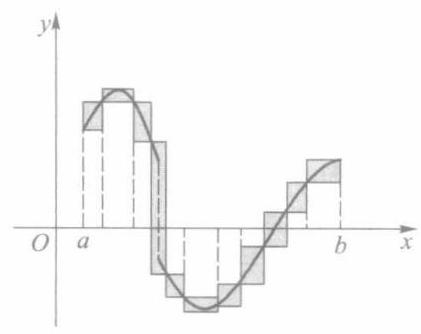
\includegraphics[width=.3\textwidth]{images/P059.jpg}
	\caption{图 $9-7$}
	\label{fig:P059}
\end{figure}

\subsection{可积函数类}

根据可积的充要条件, 我们证明下面一些类型的函数是可积的 (即可积的充分条件).

%定理 9.4
\begin{theorem}{}{the:}

\end{theorem}
 若 \(f\) 为 \(\left\lbrack  {a,b}\right\rbrack\) 上的连续函数,则 \(f\) 在 \(\left\lbrack  {a,b}\right\rbrack\) 上可积.

%证
\begin{proof}

\end{proof}
由于 \(f\) 在闭区间 \(\left\lbrack  {a,b}\right\rbrack\) 上连续,因此在 \(\left\lbrack  {a,b}\right\rbrack\) 上一致连续. 这就是说,任给 \(\varepsilon  > 0\) , 存在 \(\delta  > 0\) ,对 \(\left\lbrack  {a,b}\right\rbrack\) 中任意两点 \({x}^{\prime },{x}^{\prime \prime }\) ,只要 \(\left| {{x}^{\prime } - {x}^{\prime \prime }}\right|  < \delta\) ,便有
\[
\left| {f\left( {x}^{\prime }\right)  - f\left( {x}^{\prime \prime }\right) }\right|  < \frac{\varepsilon }{b - a}.
\]
所以只要对 \(\left\lbrack  {a,b}\right\rbrack\) 所作的分割 \(T\) 满足 \(\parallel T\parallel  < \delta\) ,在 \(T\) 所属的任一小区间 \({\Delta }_{i}\) 上,就能使 \(f\) 的振幅满足
\[
{\omega }_{i} = {M}_{i} - {m}_{i} = \mathop{\sup }\limits_{{{x}^{\prime },{x}^{\prime \prime } \in  {\Delta }_{i}}}{\left| f\left( {x}^{\prime }\right)  - f\left( {x}^{\prime \prime }\right) \right| }\footnote{此等式成立的证明留作本节习题 (第 5 题).} \leq  \frac{\varepsilon }{b - a},
\]
从而导致
\[
\mathop{\sum }\limits_{T}{\omega }_{i}\Delta {x}_{i} \leq  \frac{\varepsilon }{b - a}\mathop{\sum }\limits_{T}\Delta {x}_{i} = \varepsilon .
\]
由定理 \({9.3}^{\prime }\) 证得 \(f\) 在 \(\left\lbrack  {a,b}\right\rbrack\) 上可积.

读者应该注意到一致连续性在本定理证明中所起的重要作用.

%定理 9.5
\begin{theorem}{}{the:}

\end{theorem}
 若 \(f\) 是区间 \(\left\lbrack  {a,b}\right\rbrack\) 上只有有限个间断点的有界函数,则 \(f\) 在 \(\left\lbrack  {a,b}\right\rbrack\) 上可积.

%证
\begin{proof}

\end{proof}
不失一般性,这里只证明 \(f\) 在 \(\left\lbrack  {a,b}\right\rbrack\) 上仅有一个间断点的情形,并假设该间断点即为端点 \(b\) .

任给 \(\varepsilon  > 0\) ,取 \({\delta }^{\prime }\) 满足 \(0 < {\delta }^{\prime } < \frac{\varepsilon }{2\left( {M - m}\right) }\) ,且 \({\delta }^{\prime } < b - a\) ,其中 \(M\) 与 \(m\) 分别为 \(f\) 在 \(\left\lbrack  {a,b}\right\rbrack\) 上的上确界与下确界 (设 \(m < M\) ,否则 \(f\) 为常量函数,显然可积). 记 \(f\) 在小区间 \({\Delta }^{\prime } = \left\lbrack  {b - {\delta }^{\prime },b}\right\rbrack\) 上的振幅为 \({\omega }^{\prime }\) ,则
\[
{\omega }^{\prime }{\delta }^{\prime } < \left( {M - m}\right)  \cdot  \frac{\varepsilon }{2\left( {M - m}\right) } = \frac{\varepsilon }{2}.
\]
因为 \(f\) 在 \(\left\lbrack  {a,b - {\delta }^{\prime }}\right\rbrack\) 上连续,由定理 9.4 知 \(f\) 在 \(\left\lbrack  {a,b - {\delta }^{\prime }}\right\rbrack\) 上可积. 再由定理 \({9.3}^{\prime }\) (必要性),存在对 \(\left\lbrack  {a,b - {\delta }^{\prime }}\right\rbrack\) 的某个分割 \({T}^{\prime } = \left\{  {{\Delta }_{1},{\Delta }_{2},\cdots ,{\Delta }_{n - 1}}\right\}\) ,使得
\[
\mathop{\sum }\limits_{{T}^{\prime }}{\omega }_{i}\Delta {x}_{i} < \frac{\varepsilon }{2}.
\]
令 \({\Delta }_{n} = {\Delta }^{\prime }\) ,则 \(T = \left\{  {{\Delta }_{1},{\Delta }_{2},\cdots ,{\Delta }_{n - 1},{\Delta }_{n}}\right\}\) 是对 \(\left\lbrack  {a,b}\right\rbrack\) 的一个分割,对于 \(T\) ,有
\[
\mathop{\sum }\limits_{T}{\omega }_{i}\Delta {x}_{i} = \mathop{\sum }\limits_{{T}^{\prime }}{\omega }_{i}\Delta {x}_{i} + {\omega }^{\prime }{\delta }^{\prime } < \frac{\varepsilon }{2} + \frac{\varepsilon }{2} = \varepsilon .
\]
根据定理 \({9.3}^{\prime }\) (充分性),证得 \(f\) 在 \(\left\lbrack  {a,b}\right\rbrack\) 上可积.

%定理 9.6
\begin{theorem}{}{the:}

\end{theorem}
 若 \(f\) 是 \(\left\lbrack  {a,b}\right\rbrack\) 上的单调函数,则 \(f\) 在 \(\left\lbrack  {a,b}\right\rbrack\) 上可积.

%证
\begin{proof}

\end{proof}
设 \(f\) 为增函数,且 \(f\left( a\right)  < f\left( b\right)\) (若 \(f\left( a\right)  = f\left( b\right)\) ,则 \(f\) 为常量函数,显然可积). 对 \(\left\lbrack  {a,b}\right\rbrack\) 的任一分割 \(T\) ,由 \(f\) 的增性, \(f\) 在 \(T\) 所属的每个小区间 \({\Delta }_{i}\) 上的振幅为
\[
{\omega }_{i} = f\left( {x}_{i}\right)  - f\left( {x}_{i - 1}\right) ,
\]
于是有
\[
\mathop{\sum }\limits_{T}{\omega }_{i}\Delta {x}_{i} \leq  \mathop{\sum }\limits_{{i = 1}}^{n}\left\lbrack  {f\left( {x}_{i}\right)  - f\left( {x}_{i - 1}\right) }\right\rbrack  \parallel T\parallel
\]
\[
= \left\lbrack  {f\left( b\right)  - f\left( a\right) }\right\rbrack  \parallel T\parallel \text{ . }
\]
由此可见,任给 \(\varepsilon  > 0\) ,只要 \(\parallel T\parallel  < \frac{\varepsilon }{f\left( b\right)  - f\left( a\right) }\) ,就有
\[
\mathop{\sum }\limits_{T}{\omega }_{i}\Delta {x}_{i} < \varepsilon ,
\]
所以 \(f\) 在 \(\left\lbrack  {a,b}\right\rbrack\) 上可积.



注意, 单调函数即使有无限多个间断点, 仍不失其可积性.

%例 2
\begin{example}

\end{example}
试用两种方法证明函数
\[
f\left( x\right)  = \left\{  \begin{array}{ll} 0, & x = 0, \\  \frac{1}{n}, & \frac{1}{n + 1} < x \leq  \frac{1}{n},n = 1,2,\cdots  \end{array}\right.
\]
在区间 \(\left\lbrack  {0,1}\right\rbrack\) 上可积.

%证
\begin{proof}

\end{proof}
证法一 由于 \(f\) 是一增函数 (图 9-8),虽然它在 \(\left\lbrack  {0,1}\right\rbrack\) 上有无限多个间断点 \({x}_{n} = \frac{1}{n},n = 2,3,\cdots\) ,但由定理 9.6,仍保证它在 \(\left\lbrack  {0,1}\right\rbrack\) 上可积.

\begin{figure}
	\centering
	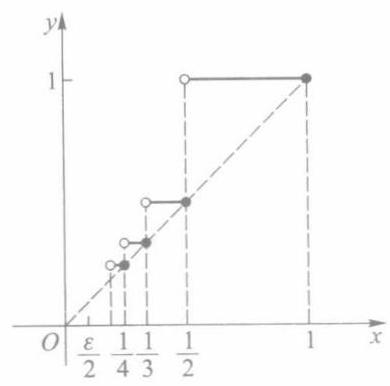
\includegraphics[width=.3\textwidth]{images/P060.jpg}
	\caption{图 $9-8$}
	\label{fig:P060}
\end{figure}

证法二 (仅利用定理 \({9.3}^{\prime }\) 和定理 9.5) 任给 \(\varepsilon  > 0\) , 由于 \(\mathop{\lim }\limits_{{n \rightarrow  \infty }}\frac{1}{n} = 0\) ,因此当 \(n\) 充分大时 \(\frac{1}{n} < \frac{\varepsilon }{2}\) ,这说明 \(f\) 在 \(\left\lbrack  {\frac{\varepsilon }{2},1}\right\rbrack\) 上只有有限个间断点. 利用定理 9.5 和定理 \({9.3}^{\prime }\) 推知 \(f\) 在 \(\left\lbrack  {\frac{\varepsilon }{2},1}\right\rbrack\) 上可积,且存在对 \(\left\lbrack  {\frac{\varepsilon }{2},1}\right\rbrack\) 的某一分割 \({T}^{\prime }\) ,使得
\[
\mathop{\sum }\limits_{{T}^{\prime }}{\omega }_{i}\Delta {x}_{i} < \frac{\varepsilon }{2}.
\]
再把小区间 \(\left\lbrack  {0,\frac{\varepsilon }{2}}\right\rbrack\) 与 \({T}^{\prime }\) 合并,成为对 \(\left\lbrack  {0,1}\right\rbrack\) 的一个分割 \(T\) . 由于 \(f\) 在 \(\left\lbrack  {0,\frac{\varepsilon }{2}}\right\rbrack\) 上的振幅 \({\omega }_{0}\) <1, 因此得到
\[
\mathop{\sum }\limits_{T}{\omega }_{i}\Delta {x}_{i} = {\omega }_{0} \cdot  \frac{\varepsilon }{2} + \mathop{\sum }\limits_{{T}^{\prime }}{\omega }_{i}\Delta {x}_{i} < \frac{\varepsilon }{2} + \frac{\varepsilon }{2} = \varepsilon .
\]
所以 \(f\) 在 \(\left\lbrack  {0,1}\right\rbrack\) 上可积.

事实上, 例 2 的第二种证法并不限于该例中的具体函数, 更一般的命题见本节习题第 4 题. 下面例 3 的证明思想与它可谓异曲同工.

%例 3
\begin{example}

\end{example}
证明黎曼函数
\[
R\left( x\right)  = \left\{  \begin{array}{ll} \frac{1}{q}, & x = \frac{p}{q}\left( {p,q \in  {\mathbf{N}}_{ + },\frac{p}{q}\text{ 为既约真分数 }}\right) , \\  0, & x = 0,1\text{ 以及 }\left( {0,1}\right) \text{ 内的无理数 } \end{array}\right.
\]
在区间 \(\left\lbrack  {0,1}\right\rbrack\) 上可积,且
\[
{\int }_{0}^{1}R\left( x\right) \mathrm{d}x = 0.
\]
分析 已知黎曼函数在 \(x = 0,1\) 以及一切无理点处连续,而在(0,1)上的一切有理点处间断. 证明它在 \(\left\lbrack  {0,1}\right\rbrack\) 上可积的直观构思如下: 如图 9-9 所示,在黎曼函数的图像中画一条水平直线 \(y = \frac{\varepsilon }{2}\) . 在此直线上方只有函数图像中有限个点,这些点所对应的自变量可被含于属于分割 \(T\) 的有限个小区间中,当 \(\parallel T\parallel\) 足够小时,这有限个小区间的总

长可为任意小; 而 \(T\) 中其余小区间上函数的振幅不大于 \(\frac{\varepsilon }{2}\) ,把这两部分相合,便可证得 \(\mathop{\sum }\limits_{T}{\omega }_{i}\Delta {x}_{i} < \varepsilon\) . 下面写出这个证明.

\begin{figure}
	\centering
	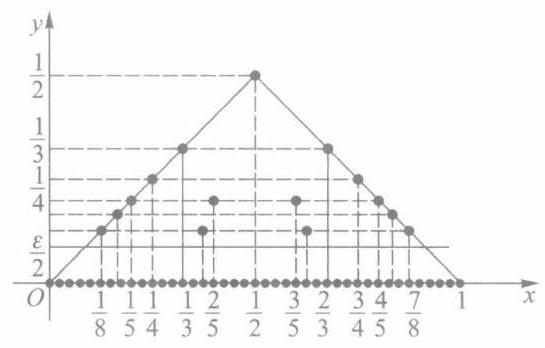
\includegraphics[width=.3\textwidth]{images/P061.jpg}
	\caption{图 $9-9$}
	\label{fig:P061}
\end{figure}

%证
\begin{proof}

\end{proof}
任给 \(\varepsilon  > 0\) ,在 \(\left\lbrack  {0,1}\right\rbrack\) 上使得 \(\frac{1}{q} > \frac{\varepsilon }{2}\) 的有理点 \(\frac{p}{q}\) 只有有限个,设它们为 \({r}_{1},\cdots ,{r}_{k}\) . 现对 \(\left\lbrack  {0,1}\right\rbrack\) 作分割 \(T = \left\{  {{\Delta }_{1},{\Delta }_{2},\cdots ,{\Delta }_{n}}\right\}\) ,使 \(\parallel T\parallel  < \frac{\varepsilon }{2k}\) ,并把 \(T\) 中所有小区间分为 \(\left\{  {{\Delta }_{i}^{\prime } \mid  i = }\right.\)  \(1,2,\cdots ,m\}\) 和 \(\left\{  {{\Delta }_{i}^{\prime \prime } \mid  i = 1,2,\cdots ,n - m}\right\}\) 两类. 其中 \(\left\{  {\Delta }_{i}^{\prime }\right\}\) 为含有 \(\left\{  {{r}_{i} \mid  i = 1,2,\cdots ,k}\right\}\) 中点的所有小区间,这类小区间的个数 \(m \leq  {2k}\) (当所有 \({r}_{i}\) 恰好都是 \(T\) 的分割点时才有 \(m = {2k}\) ); 而 \(\left\{  {\Delta }_{i}^{\prime \prime }\right\}\) 为 \(T\) 中所有其余不含 \(\left\{  {r}_{i}\right\}\) 中点的小区间. 由于 \(f\) 在 \({\Delta }_{i}^{\prime }\) 上的振幅 \({\omega }_{i}^{\prime } \leq  \frac{1}{2}\) ,于是
\[
\mathop{\sum }\limits_{{i = 1}}^{m}{\omega }_{i}^{\prime }\Delta {x}_{i}^{\prime } \leq  \frac{1}{2}\mathop{\sum }\limits_{{i = 1}}^{m}\Delta {x}_{i}^{\prime } \leq  \frac{1}{2} \cdot  {2k}\parallel T\parallel  < \frac{\varepsilon }{2};
\]
而 \(f\) 在 \({\Delta }_{i}^{\prime \prime }\) 上的振幅 \({\omega }_{i}^{\prime \prime } \leq  \frac{\varepsilon }{2}\) ,于是
\[
\mathop{\sum }\limits_{{i = 1}}^{{n - m}}{\omega }_{i}^{\prime \prime }\Delta {x}_{i}^{\prime \prime } \leq  \frac{\varepsilon }{2}\mathop{\sum }\limits_{{i = 1}}^{{n - m}}\Delta {x}_{i}^{\prime \prime } < \frac{\varepsilon }{2}.
\]
把这两部分合起来, 便证得
\[
\mathop{\sum }\limits_{{i = 1}}^{n}{\omega }_{i}\Delta {x}_{i} = \mathop{\sum }\limits_{{i = 1}}^{m}{\omega }_{i}^{\prime }\Delta {x}_{i}^{\prime } + \mathop{\sum }\limits_{{i = 1}}^{{n - m}}{\omega }_{i}^{\prime \prime }\Delta {x}_{i}^{\prime \prime } < \varepsilon ,
\]
即 \(f\) 在 \(\left\lbrack  {0,1}\right\rbrack\) 上可积.

因为已经证得 \(f\) 在 \(\left\lbrack  {0,1}\right\rbrack\) 上可积,所以当取 \({\xi }_{i}\) 全为无理点时,使 \(f\left( {\xi }_{i}\right)  = 0\) ,从而
\[
{\int }_{0}^{1}R\left( x\right) \mathrm{d}x = \mathop{\lim }\limits_{{\parallel T\parallel  \rightarrow  0}}\mathop{\sum }\limits_{{i = 1}}^{n}R\left( {\xi }_{i}\right) \Delta {x}_{i} = 0.
\]
\subsection{习题 9.3}

1. 证明: 若 \({T}^{\prime }\) 是 \(T\) 增加若干个分点后所得的分割,则 \(\mathop{\sum }\limits_{{T}^{\prime }}{\omega }_{i}^{\prime }\Delta {x}_{i}^{\prime } \leq  \mathop{\sum }\limits_{T}{\omega }_{i}\Delta {x}_{i}\) .

2. 证明: 若 \(f\) 在 \(\left\lbrack  {a,b}\right\rbrack\) 上可积, \(\left\lbrack  {\alpha ,\beta }\right\rbrack   \subset  \left\lbrack  {a,b}\right\rbrack\) ,则 \(f\) 在 \(\left\lbrack  {\alpha ,\beta }\right\rbrack\) 上也可积.

3. 设 \(f,g\) 均为定义在 \(\left\lbrack  {a,b}\right\rbrack\) 上的有界函数,仅在有限个点处 \(f\left( x\right)  \neq  g\left( x\right)\) . 证明: 若 \(f\) 在 \(\left\lbrack  {a,b}\right\rbrack\) 上可积,则 \(g\) 在 \(\left\lbrack  {a,b}\right\rbrack\) 上也可积,且 \({\int }_{a}^{b}f\left( x\right) \mathrm{d}x = {\int }_{a}^{b}g\left( x\right) \mathrm{d}x\) .

4. 设 \(f\) 在 \(\left\lbrack  {a,b}\right\rbrack\) 上有界, \(\left\{  {a}_{n}\right\}   \subset  \left\lbrack  {a,b}\right\rbrack  ,\mathop{\lim }\limits_{{n \rightarrow  \infty }}{a}_{n} = c\) . 证明: 若 \(f\) 在 \(\left\lbrack  {a,b}\right\rbrack\) 上只有 \({a}_{n}\left( {n = 1,2,\cdots }\right)\) 为其间断点,则 \(f\) 在 \(\left\lbrack  {a,b}\right\rbrack\) 上可积.

5. 证明: 若 \(f\) 在区间 \(\Delta\) 上有界,则
\[
\mathop{\sup }\limits_{{x \in  \Delta }}f\left( x\right)  - \mathop{\inf }\limits_{{x \in  \Delta }}f\left( x\right)  = \mathop{\sup }\limits_{{{x}^{\prime },{x}^{\prime \prime } \in  \Delta }}\left| {f\left( {x}^{\prime }\right)  - f\left( {x}^{\prime \prime }\right) }\right| .
\]
6. 证明函数
\[
f\left( x\right)  = \left\{  \begin{array}{ll} 0, & x = 0, \\  \frac{1}{x} - \left\lbrack  \frac{1}{x}\right\rbrack  , & x \in  (0,1\rbrack  \end{array}\right.
\]
在 \(\left\lbrack  {0,1}\right\rbrack\) 上可积.

7. 设函数 \(f\) 在 \(\left\lbrack  {a,b}\right\rbrack\) 上有定义,且对于任给的 \(\varepsilon  > 0\) ,存在 \(\left\lbrack  {a,b}\right\rbrack\) 上的可积函数 \(g\) ,使得
\[
\left| {f\left( x\right)  - g\left( x\right) }\right|  < \varepsilon ,\;x \in  \left\lbrack  {a,b}\right\rbrack  .
\]
证明 \(f\) 在 \(\left\lbrack  {a,b}\right\rbrack\) 上可积.

\section{定积分的性质}

\subsection{定积分的基本性质}

性质 1 若 \(f\) 在 \(\left\lbrack  {a,b}\right\rbrack\) 上可积, \(k\) 为常数,则 \({kf}\) 在 \(\left\lbrack  {a,b}\right\rbrack\) 上也可积,且
\[
{\int }_{a}^{b}{kf}\left( x\right) \mathrm{d}x = k{\int }_{a}^{b}f\left( x\right) \mathrm{d}x. \tag{1}
\]
%证
\begin{proof}

\end{proof}
当 \(k = 0\) 时结论显然成立.

当 \(k \neq  0\) 时,由于
\[
\left| {\mathop{\sum }\limits_{{i = 1}}^{n}{kf}\left( {\xi }_{i}\right) \Delta {x}_{i} - {kJ}}\right|  = \left| k\right|  \cdot  \left| {\mathop{\sum }\limits_{{i = 1}}^{n}f\left( {\xi }_{i}\right) \Delta {x}_{i} - J}\right| ,
\]
其中 \(J = {\int }_{a}^{b}f\left( x\right) \mathrm{d}x\) ,因此当 \(f\) 在 \(\left\lbrack  {a,b}\right\rbrack\) 上可积时,由定义,任给 \(\varepsilon  > 0\) ,存在 \(\delta  > 0\) ,当 \(\parallel T\parallel  < \delta\) 时,
\[
\left| {\mathop{\sum }\limits_{{i = 1}}^{n}f\left( {\xi }_{i}\right) \Delta {x}_{i} - J}\right|  < \frac{\varepsilon }{\left| k\right| },
\]
从而
\[
\left| {\mathop{\sum }\limits_{{i = 1}}^{n}{kf}\left( {\xi }_{i}\right) \Delta {x}_{i} - {kJ}}\right|  < \varepsilon .
\]
即 \({kf}\) 在 \(\left\lbrack  {a,b}\right\rbrack\) 上可积,且
\[
{\int }_{a}^{b}{kf}\left( x\right) \mathrm{d}x = {kJ} = k{\int }_{a}^{b}f\left( x\right) \mathrm{d}x.
\]
性质 2 若 \(f,g\) 都在 \(\left\lbrack  {a,b}\right\rbrack\) 上可积,则 \(f \pm  g\) 在 \(\left\lbrack  {a,b}\right\rbrack\) 上也可积,且
\[
{\int }_{a}^{b}\left\lbrack  {f\left( x\right)  \pm  g\left( x\right) }\right\rbrack  \mathrm{d}x = {\int }_{a}^{b}f\left( x\right) \mathrm{d}x \pm  {\int }_{a}^{b}g\left( x\right) \mathrm{d}x. \tag{2}
\]
证明与性质 1 类同, 留给读者.

性质 1 与性质 2 是定积分的线性性质, 合起来即为
\[
{\int }_{a}^{b}\left\lbrack  {{\alpha f}\left( x\right)  + {\beta g}\left( x\right) }\right\rbrack  \mathrm{d}x = \alpha {\int }_{a}^{b}f\left( x\right) \mathrm{d}x + \beta {\int }_{a}^{b}g\left( x\right) \mathrm{d}x,
\]
其中 \(\alpha ,\beta\) 为常数.

性质 3 若 \(f,g\) 都在 \(\left\lbrack  {a,b}\right\rbrack\) 上可积,则 \(f \cdot  g\) 在 \(\left\lbrack  {a,b}\right\rbrack\) 上也可积.

%证
\begin{proof}

\end{proof}
由 \(f,g\) 都在 \(\left\lbrack  {a,b}\right\rbrack\) 上可积,从而都有界,设
\[
A = \mathop{\sup }\limits_{{x \in  \left\lbrack  {a,b}\right\rbrack  }}\left| {f\left( x\right) }\right| ,\;B = \mathop{\sup }\limits_{{x \in  \left\lbrack  {a,b}\right\rbrack  }}\left| {g\left( x\right) }\right| ,
\]
且 \(A > 0,B > 0\) (否则 \(f,g\) 中至少有一个恒为零值函数,于是 \(f \cdot  g\) 亦为零值函数,结论显然成立).

任给 \(\varepsilon  > 0\) ,由 \(f,g\) 可积,必分别存在分割 \({T}_{1},{T}_{2}\) ,使得
\[
\mathop{\sum }\limits_{{T}_{1}}{\omega }_{1,i}^{f}\Delta {x}_{1,i} < \frac{\varepsilon }{2B},\;\mathop{\sum }\limits_{{T}_{2}}{\omega }_{2,i}^{g}\Delta {x}_{2,i} < \frac{\varepsilon }{2A}.
\]
令 \(T = {T}_{1} + {T}_{2}\) (表示把 \({T}_{1},{T}_{2}\) 的所有分割点合并而成的一个新的分割 \(T\) ). 对于 \(\left\lbrack  {a,b}\right\rbrack\) 上 \(T\) 所属的每一个 \({\Delta }_{i}\) ,有
\[
{\omega }_{i}^{f \cdot  g} = \mathop{\sup }\limits_{{{x}^{\prime },{x}^{\prime \prime } \in  {\Delta }_{i}}}\left| {f\left( {x}^{\prime }\right) g\left( {x}^{\prime }\right)  - f\left( {x}^{\prime \prime }\right) g\left( {x}^{\prime \prime }\right) }\right|
\]
\[
\leq  \mathop{\sup }\limits_{{{x}^{\prime },{x}^{\prime \prime } \in  {\Delta }_{i}}}\left\lbrack  {\left| {g\left( {x}^{\prime }\right) }\right|  \cdot  \left| {f\left( {x}^{\prime }\right)  - f\left( {x}^{\prime \prime }\right) }\right|  + \left| {f\left( {x}^{\prime \prime }\right) }\right|  \cdot  \left| {g\left( {x}^{\prime }\right)  - g\left( {x}^{\prime \prime }\right) }\right| }\right\rbrack
\]
\[
\leq  B{\omega }_{i}^{f} + A{\omega }_{i}^{g}.
\]
利用习题 9.3 的第 1 题,可知
\[
\mathop{\sum }\limits_{T}{\omega }_{i}^{f \cdot  g}\Delta {x}_{i} \leq  B\mathop{\sum }\limits_{T}{\omega }_{i}^{f}\Delta {x}_{i} + A\mathop{\sum }\limits_{T}{\omega }_{i}^{g}\Delta {x}_{i}
\]
\[
\leq  B\mathop{\sum }\limits_{{T}_{1}}{\omega }_{1,i}^{f}\Delta {x}_{1,i} + A\mathop{\sum }\limits_{{T}_{2}}{\omega }_{2,i}^{g}\Delta {x}_{2,i}
\]
\[
< B \cdot  \frac{\varepsilon }{2B} + A \cdot  \frac{\varepsilon }{2A} = \varepsilon ,
\]
这就证得 \(f \cdot  g\) 在 \(\left\lbrack  {a,b}\right\rbrack\) 上可积.

注意,在一般情形下, \({\int }_{a}^{b}f\left( x\right) g\left( x\right) \mathrm{d}x \neq  {\int }_{a}^{b}f\left( x\right) \mathrm{d}x \cdot  {\int }_{a}^{b}g\left( x\right) \mathrm{d}x\) .

性质 \({4f}\) 在 \(\left\lbrack  {a,b}\right\rbrack\) 上可积的充要条件是: 任给 \(c \in  \left( {a,b}\right) ,f\) 在 \(\left\lbrack  {a,c}\right\rbrack\) 与 \(\left\lbrack  {c,b}\right\rbrack\) 上都可积. 此时又有等式
\[
{\int }_{a}^{b}f\left( x\right) \mathrm{d}x = {\int }_{a}^{c}f\left( x\right) \mathrm{d}x + {\int }_{c}^{b}f\left( x\right) \mathrm{d}x. \tag{3}
\]
%证
\begin{proof}

\end{proof}
充分性 由于 \(f\) 在 \(\left\lbrack  {a,c}\right\rbrack\) 与 \(\left\lbrack  {c,b}\right\rbrack\) 上都可积,故任给 \(\varepsilon  > 0\) ,分别存在对 \(\left\lbrack  {a,c}\right\rbrack\) 与 \(\left\lbrack  {c,b}\right\rbrack\) 的分割 \({T}^{\prime }\) 与 \({T}^{\prime \prime }\) ,使得
\[
\mathop{\sum }\limits_{{T}^{\prime }}{\omega }_{i}^{\prime }\Delta {x}_{i}^{\prime } < \frac{\varepsilon }{2},\;\mathop{\sum }\limits_{{T}^{\prime \prime }}{\omega }_{i}^{\prime \prime }\Delta {x}_{i}^{\prime \prime } < \frac{\varepsilon }{2}.
\]
现令 \(T = {T}^{\prime } + {T}^{\prime \prime }\) ,它是对 \(\left\lbrack  {a,b}\right\rbrack\) 的一个分割,且有
\[
\mathop{\sum }\limits_{T}{\omega }_{i}\Delta {x}_{i} = \mathop{\sum }\limits_{{T}^{\prime }}{\omega }_{i}^{\prime }\Delta {x}_{i}^{\prime } + \mathop{\sum }\limits_{{T}^{\prime \prime }}{\omega }_{i}^{\prime \prime }\Delta {x}_{i}^{\prime \prime } < \varepsilon .
\]
由此证得 \(f\) 在 \(\left\lbrack  {a,b}\right\rbrack\) 上可积.

必要性 已知 \(f\) 在 \(\left\lbrack  {a,b}\right\rbrack\) 上可积,故任给 \(\varepsilon  > 0\) ,存在对 \(\left\lbrack  {a,b}\right\rbrack\) 的某分割 \(T\) ,使得 \(\mathop{\sum }\limits_{T}{\omega }_{i}\Delta {x}_{i} < \varepsilon\) . 在 \(T\) 上再增加一个分点 \(c\) ,得到一个新的分割 \({T}^{ * }\) . 由习题 9.3 的第 1 题,又有
\[
\mathop{\sum }\limits_{{T}^{ * }}{\omega }_{i}^{ * }\Delta {x}_{i}^{ * } \leq  \mathop{\sum }\limits_{T}{\omega }_{i}\Delta {x}_{i} < \varepsilon .
\]
分割 \({T}^{ * }\) 在 \(\left\lbrack  {a,c}\right\rbrack\) 和 \(\left\lbrack  {c,b}\right\rbrack\) 上的部分分别构成对 \(\left\lbrack  {a,c}\right\rbrack\) 和 \(\left\lbrack  {c,b}\right\rbrack\) 的分割,记为 \({T}^{\prime }\) 和 \({T}^{\prime \prime }\) ,则有
\[
\mathop{\sum }\limits_{{T}^{\prime }}{\omega }_{i}^{\prime }\Delta {x}_{i}^{\prime } \leq  \mathop{\sum }\limits_{{T}^{ * }}{\omega }_{i}^{ * }\Delta {x}_{i}^{ * } < \varepsilon ,
\]
\[
\mathop{\sum }\limits_{{T}^{\prime \prime }}{\omega }_{i}^{\prime \prime }\Delta {x}_{i}^{\prime \prime } \leq  \mathop{\sum }\limits_{{T}^{ * }}{\omega }_{i}^{ * }\Delta {x}_{i}^{ * } < \varepsilon .
\]
这就证得 \(f\) 在 \(\left\lbrack  {a,c}\right\rbrack\) 与 \(\left\lbrack  {c,b}\right\rbrack\) 上都可积.

在证得上面结果的基础上最后来证明等式 (3). 为此对 \(\left\lbrack  {a,b}\right\rbrack\) 作分割 \(T\) ,恒使点 \(c\) 为其中的一个分点,这时 \(T\) 在 \(\left\lbrack  {a,c}\right\rbrack\) 与 \(\left\lbrack  {c,b}\right\rbrack\) 上的部分各自构成对 \(\left\lbrack  {a,c}\right\rbrack\) 与 \(\left\lbrack  {c,b}\right\rbrack\) 的分割, 分别记为 \({T}^{\prime }\) 与 \({T}^{\prime \prime }\) . 由于
\[
\mathop{\sum }\limits_{T}f\left( {\xi }_{i}\right) \Delta {x}_{i} = \mathop{\sum }\limits_{{T}^{\prime }}f\left( {\xi }_{i}^{\prime }\right) \Delta {x}_{i}^{\prime } + \mathop{\sum }\limits_{{T}^{\prime \prime }}f\left( {\xi }_{i}^{\prime \prime }\right) \Delta {x}_{i}^{\prime \prime },
\]
因此当 \(\parallel T\parallel  \rightarrow  0\) (同时有 \(\begin{Vmatrix}{T}^{\prime }\end{Vmatrix} \rightarrow  0,\begin{Vmatrix}{T}^{\prime \prime }\end{Vmatrix} \rightarrow  0\) ) 时,对上式取极限,就得到 (3) 式成立.

性质 4 及公式 (3) 称为关于积分区间的可加性. 当 \(f\left( x\right)  \geq  0\) 时,(3) 式的几何意义就是曲边梯形面积的可加性. 如图9-10所示, 曲边梯形 AabB 的面积等于曲边梯形 AacC 的面积与 \({CcbB}\) 的面积之和.

\begin{figure}
	\centering
	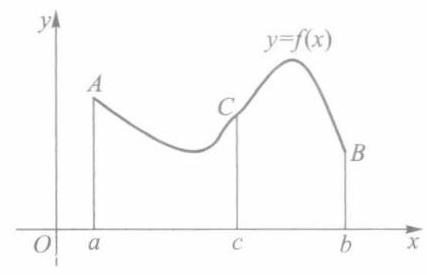
\includegraphics[width=.3\textwidth]{images/P062.jpg}
	\caption{图 $9-10$}
	\label{fig:P062}
\end{figure}

按定积分的定义,记号 \({\int }_{a}^{b}f\left( x\right) \mathrm{d}x\) 只有当 \(a < b\) 时才有意义,而当 \(a = b\) 或 \(a > b\) 时本来是没有意义的. 但为了运用上的方便, 对它作如下规定.

规定 1 当 \(a = b\) 时,令 \({\int }_{a}^{a}f\left( x\right) \mathrm{d}x = 0\) .

规定 2 当 \(a > b\) 时,令 \({\int }_{a}^{b}f\left( x\right) \mathrm{d}x =  - {\int }_{b}^{a}f\left( x\right) \mathrm{d}x\) .

有了这些规定之后,等式 (3) 对于 \(a,b,c\) 的任何大小顺序都能成立. 例如,当 \(a < b < c\) 时,只要 \(f\) 在 \(\left\lbrack  {a,c}\right\rbrack\) 上可积,则有
\[
{\int }_{a}^{c}f\left( x\right) \mathrm{d}x + {\int }_{c}^{b}f\left( x\right) \mathrm{d}x = \left( {{\int }_{a}^{b}f\left( x\right) \mathrm{d}x + {\int }_{b}^{c}f\left( x\right) \mathrm{d}x}\right)  - {\int }_{b}^{c}f\left( x\right) \mathrm{d}x
\]
\[
= {\int }_{a}^{b}f\left( x\right) \mathrm{d}x.
\]
性质 5 设 \(f\) 为 \(\left\lbrack  {a,b}\right\rbrack\) 上的可积函数. 若 \(f\left( x\right)  \geq  0,x \in  \left\lbrack  {a,b}\right\rbrack\) ,则
\[
{\int }_{a}^{b}f\left( x\right) \mathrm{d}x \geq  0. \tag{4}
\]
%证
\begin{proof}

\end{proof}
由于在 \(\left\lbrack  {a,b}\right\rbrack\) 上 \(f\left( x\right)  \geq  0\) ,因此 \(f\) 的任一积分和都为非负. 由 \(f\) 在 \(\left\lbrack  {a,b}\right\rbrack\) 上可积, 则有
\[
{\int }_{a}^{b}f\left( x\right) \mathrm{d}x = \mathop{\lim }\limits_{{\parallel T\parallel  \rightarrow  0}}\mathop{\sum }\limits_{{i = 1}}^{n}f\left( {\xi }_{i}\right) \Delta {x}_{i} \geq  0.
\]
推论 (积分不等式性) 若 \(f\) 与 \(g\) 为 \(\left\lbrack  {a,b}\right\rbrack\) 上的两个可积函数,且 \(f\left( x\right)  \leq  g\left( x\right) ,x \in\)  \(\left\lbrack  {a,b}\right\rbrack\) ,则有
\[
{\int }_{a}^{b}f\left( x\right) \mathrm{d}x \leq  {\int }_{a}^{b}g\left( x\right) \mathrm{d}x. \tag{5}
\]
%证
\begin{proof}

\end{proof}
令 \(F\left( x\right)  = g\left( x\right)  - f\left( x\right)  \geq  0,x \in  \left\lbrack  {a,b}\right\rbrack\) ,由性质 2 知道 \(F\) 在 \(\left\lbrack  {a,b}\right\rbrack\) 上可积,且由性质 5 推得
\[
0 \leq  {\int }_{a}^{b}F\left( x\right) \mathrm{d}x = {\int }_{a}^{b}g\left( x\right) \mathrm{d}x - {\int }_{a}^{b}f\left( x\right) \mathrm{d}x,
\]
不等式 (5) 得证.

性质 6 若 \(f\) 在 \(\left\lbrack  {a,b}\right\rbrack\) 上可积,则 \(\left| f\right|\) 在 \(\left\lbrack  {a,b}\right\rbrack\) 上也可积,且
\[
\left| {{\int }_{a}^{b}f\left( x\right) \mathrm{d}x}\right|  \leq  {\int }_{a}^{b}\left| {f\left( x\right) }\right| \mathrm{d}x. \tag{6}
\]
%证
\begin{proof}

\end{proof}
由于 \(f\) 在 \(\left\lbrack  {a,b}\right\rbrack\) 上可积,故任给 \(\varepsilon  > 0\) ,存在某分割 \(T\) ,使得 \(\mathop{\sum }\limits_{T}{\omega }_{i}^{f}\Delta {x}_{i} < \varepsilon\) . 由绝对值不等式
\[
\left| \right| f\left( {x}^{\prime }\right) \left| -\right| f\left( {x}^{\prime \prime }\right) \left| \right|  \leq  \left| {f\left( {x}^{\prime }\right)  - f\left( {x}^{\prime \prime }\right) }\right| ,
\]
可得 \({\omega }_{i}^{\left| f\right| } \leq  {\omega }_{i}^{f}\) ,于是有
\[
\mathop{\sum }\limits_{T}{\omega }_{i}^{\left| f\right| }\Delta {x}_{i} \leq  \mathop{\sum }\limits_{T}{\omega }_{i}^{f}\Delta {x}_{i} < \varepsilon .
\]
从而证得 \(\left| f\right|\) 在 \(\left\lbrack  {a,b}\right\rbrack\) 上可积.

再由不等式- \(\left| {f\left( x\right) }\right|  \leq  f\left( x\right)  \leq  \left| {f\left( x\right) }\right|\) ,应用性质 5 (推论),即证得不等式 (6) 成立.

%注
\begin{remark}

\end{remark}
这个性质的逆命题一般不成立. 例如
\[
f\left( x\right)  = \begin{cases} 1, & x\text{ 为有理数, } \\   - 1, & x\text{ 为无理数 } \end{cases}
\]
在 \(\left\lbrack  {0,1}\right\rbrack\) 上不可积 (类似于狄利克雷函数); 但 \(\left| {f\left( x\right) }\right|  \equiv  1\) ,它在 \(\left\lbrack  {0,1}\right\rbrack\) 上可积.

%例 1
\begin{example}

\end{example}
求 \({\int }_{-1}^{1}f\left( x\right) \mathrm{d}x\) ,其中
\[
f\left( x\right)  = \left\{  \begin{array}{ll} {2x} - 1, &  - 1 \leq  x < 0, \\  {\mathrm{e}}^{-x}, & 0 \leq  x \leq  1. \end{array}\right.
\]
%解
\begin{solution}

\end{solution}
对于分段函数的定积分, 通常利用积分区间可加性来计算, 即
\[
{\int }_{-1}^{1}f\left( x\right) \mathrm{d}x = {\int }_{-1}^{0}f\left( x\right) \mathrm{d}x + {\int }_{0}^{1}f\left( x\right) \mathrm{d}x
\]
\[
= {\int }_{-1}^{0}\left( {{2x} - 1}\right) \mathrm{d}x + {\int }_{0}^{1}{\mathrm{e}}^{-x}\mathrm{\;d}x
\]
\[
= {\left. \left( {x}^{2} - x\right) \right| }_{-1}^{0} + {\left. \left( -{\mathrm{e}}^{-x}\right) \right| }_{0}^{1}
\]
\[
=  - 2 - {\mathrm{e}}^{-1} + 1 =  - \left( {{\mathrm{e}}^{-1} + 1}\right) \text{ . }
\]
%注
\begin{remark}

\end{remark}
1 上述解法中取 \({\int }_{-1}^{0}f\left( x\right) \mathrm{d}x = {\int }_{-1}^{0}\left( {{2x} - 1}\right) \mathrm{d}x\) ,其中被积函数在 \(x = 0\) 处的值已由原来的 \(f\left( 0\right)  = {\left. {\mathrm{e}}^{-x}\right| }_{x = 0} = 1\) 改为 \({\left. \left( 2x - 1\right) \right| }_{x = 0} =  - 1\) ,由习题 9.3 的第 3 题知道这一改动并不影响 \(f\) 在 \(\left\lbrack  {-1,0}\right\rbrack\) 上的可积性和定积分的值.

%注
\begin{remark}

\end{remark}
2 如果要求直接在 \(\left\lbrack  {-1,1}\right\rbrack\) 上使用牛顿一莱布尼茨公式来计算 \({\int }_{-1}^{1}f\left( x\right) \mathrm{d}x =\)  \(F\left( 1\right)  - F\left( {-1}\right)\) ,这时 \(F\left( x\right)\) 应取怎样的函数? 读者可对照习题 9.2 的第 3 题来回答.

%例 2
\begin{example}

\end{example}
证明: 若 \(f\) 在 \(\left\lbrack  {a,b}\right\rbrack\) 上连续,且 \(f\left( x\right)  \geq  0,{\int }_{a}^{b}f\left( x\right) \mathrm{d}x = 0\) ,则 \(f\left( x\right)  \equiv  0,x \in  \left\lbrack  {a,b}\right\rbrack\) .

%证
\begin{proof}

\end{proof}
用反证法. 倘若有某 \({x}_{0} \in  \left\lbrack  {a,b}\right\rbrack\) ,使 \(f\left( {x}_{0}\right)  > 0\) ,则由连续函数的局部保号性,存在 \({x}_{0}\) 的某邻域 \(\left( {{x}_{0} - \delta ,{x}_{0} + \delta }\right)\) (当 \({x}_{0} = a\) 或 \({x}_{0} = b\) 时,则为右邻域或左邻域),使在其中 \(f\left( x\right)  \geq  \frac{f\left( {x}_{0}\right) }{2} > 0\) . 由性质 4 和性质 5 推知
\[
{\int }_{a}^{b}f\left( x\right) \mathrm{d}x = {\int }_{a}^{{x}_{0} - \delta }f\left( x\right) \mathrm{d}x + {\int }_{{x}_{0} - \delta }^{{x}_{0} + \delta }f\left( x\right) \mathrm{d}x + {\int }_{{x}_{0} + \delta }^{b}f\left( x\right) \mathrm{d}x
\]
\[
\geq  0 + {\int }_{{x}_{0} - \delta }^{{x}_{0} + \delta }\frac{f\left( {x}_{0}\right) }{2}\mathrm{\;d}x + 0 = f\left( {x}_{0}\right) \delta  > 0,
\]
这与假设 \({\int }_{a}^{b}f\left( x\right) \mathrm{d}x = 0\) 相矛盾. 所以 \(f\left( x\right)  \equiv  0,x \in  \left\lbrack  {a,b}\right\rbrack\) .

%注
\begin{remark}

\end{remark}
从此例证明中看到,即使 \(f\) 为一非负可积函数,只要它在某一点 \({x}_{0}\) 处连续,且 \(f\left( {x}_{0}\right)  > 0\) ,则必有 \({\int }_{a}^{b}f\left( x\right) \mathrm{d}x > 0\) . (至于可积函数必有连续点,这是一个较难证明的命题, 读者可参阅习题 9.6 的第 7 题. )

\subsection{积分中值定理}

%定理 9.7
\begin{theorem}{}{the:}

\end{theorem}
 (积分第一中值定理) 若 \(f\) 在 \(\left\lbrack  {a,b}\right\rbrack\) 上连续,则至少存在一点 \(\xi  \in  \left\lbrack  {a,b}\right\rbrack\) , 使得
\[
{\int }_{a}^{b}f\left( x\right) \mathrm{d}x = f\left( \xi \right) \left( {b - a}\right) . \tag{7}
\]
%证
\begin{proof}

\end{proof}
由于 \(f\) 在 \(\left\lbrack  {a,b}\right\rbrack\) 上连续,因此存在最大值 \(M\) 和最小值 \(m\) . 由
\[
m \leq  f\left( x\right)  \leq  M,\;x \in  \left\lbrack  {a,b}\right\rbrack  ,
\]
使用积分不等式性质得到
\[
m\left( {b - a}\right)  \leq  {\int }_{a}^{b}f\left( x\right) \mathrm{d}x \leq  M\left( {b - a}\right) ,
\]
或
\[
m \leq  \frac{1}{b - a}{\int }_{a}^{b}f\left( x\right) \mathrm{d}x \leq  M.
\]
再由连续函数的介值性,至少存在一点 \(\xi  \in  \left\lbrack  {a,b}\right\rbrack\) ,使得
\[
f\left( \xi \right)  = \frac{1}{b - a}{\int }_{a}^{b}f\left( x\right) \mathrm{d}x,
\]
 (7')

这就证得 (7) 式成立.

积分第一中值定理的几何意义如图 9-11 所示,若 \(f\) 在 \(\left\lbrack  {a,b}\right\rbrack\) 上非负连续,则 \(y =\)  \(f\left( x\right)\) 在 \(\left\lbrack  {a,b}\right\rbrack\) 上的曲边梯形面积等于以 \(\left( {7}^{\prime }\right)\) 所示的 \(f\left( \xi \right)\) 为高, \(\left\lbrack  {a,b}\right\rbrack\) 为底的矩形面积. 而 \(\frac{1}{b - a}{\int }_{a}^{b}f\left( x\right) \mathrm{d}x\) 则可理解为 \(f\left( x\right)\) 在区间 \(\left\lbrack  {a,b}\right\rbrack\) 上所有函数值的平均值. 这是通常有限个数的算术平均值的推广.

\begin{figure}
	\centering
	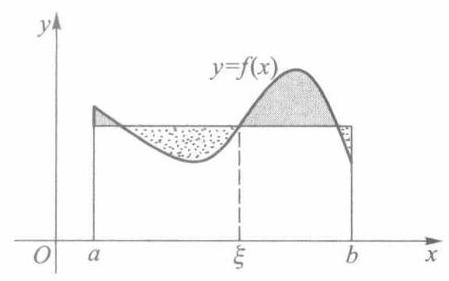
\includegraphics[width=.3\textwidth]{images/P063.jpg}
	\caption{图 $9-11$}
	\label{fig:P063}
\end{figure}

%例 3
\begin{example}

\end{example}
试求 \(f\left( x\right)  = \sin x\) 在 \(\left\lbrack  {0,\pi }\right\rbrack\) 上的平均值.

%解
\begin{solution}

\end{solution}
所求平均值为
\[
f\left( \xi \right)  = \frac{1}{\pi }{\int }_{0}^{\pi }\sin x\mathrm{\;d}x =  - {\left. \frac{1}{\pi }\cos x\right| }_{0}^{\pi } = \frac{2}{\pi }. \tag{0}
\]
%定理 9.8
\begin{theorem}{}{the:}

\end{theorem}
 (推广的积分第一中值定理) 若 \(f\) 与 \(g\) 都在 \(\left\lbrack  {a,b}\right\rbrack\) 上连续,且 \(g\left( x\right)\) 在 \(\left\lbrack  {a,b}\right\rbrack\) 上不变号,则至少存在一点 \(\xi  \in  \left\lbrack  {a,b}\right\rbrack\) ,使得
\[
{\int }_{a}^{b}f\left( x\right) g\left( x\right) \mathrm{d}x = f\left( \xi \right) {\int }_{a}^{b}g\left( x\right) \mathrm{d}x. \tag{8}
\]
(当 \(g\left( x\right)  \equiv  1\) 时,即为定理 9.7.)

%证
\begin{proof}

\end{proof}
不妨设 \(g\left( x\right)  \geq  0,x \in  \left\lbrack  {a,b}\right\rbrack\) . 这时有
\[
{mg}\left( x\right)  \leq  f\left( x\right) g\left( x\right)  \leq  {Mg}\left( x\right) ,x \in  \left\lbrack  {a,b}\right\rbrack  ,
\]
其中 \(M,m\) 分别为 \(f\) 在 \(\left\lbrack  {a,b}\right\rbrack\) 上的最大、最小值. 由定积分的不等式性质,得到
\[
m{\int }_{a}^{b}g\left( x\right) \mathrm{d}x \leq  {\int }_{a}^{b}f\left( x\right) g\left( x\right) \mathrm{d}x \leq  M{\int }_{a}^{b}g\left( x\right) \mathrm{d}x.
\]
若 \({\int }_{a}^{b}g\left( x\right) \mathrm{d}x = 0\) ,则由上式知 \({\int }_{a}^{b}f\left( x\right) g\left( x\right) \mathrm{d}x = 0\) ,从而对任何 \(\xi  \in  \left\lbrack  {a,b}\right\rbrack  ,\left( 8\right)\) 式都成立. 若 \({\int }_{a}^{b}g\left( x\right) \mathrm{d}x > 0\) ,则得
\[
m \leq  \frac{{\int }_{a}^{b}f\left( x\right) g\left( x\right) \mathrm{d}x}{{\int }_{a}^{b}g\left( x\right) \mathrm{d}x} \leq  M.
\]
由连续函数的介值性,必至少有一点 \(\xi  \in  \left\lbrack  {a,b}\right\rbrack\) ,使得
\[
f\left( \xi \right)  = \frac{{\int }_{a}^{b}f\left( x\right) g\left( x\right) \mathrm{d}x}{{\int }_{a}^{b}g\left( x\right) \mathrm{d}x},
\]
这就证得 (8) 式成立.

%注
\begin{remark}

\end{remark}
事实上,定理 9.7 和定理 9.8 中的中值点 \(\xi\) 必能在开区间(a, b)上取得 (证明留作习题).

%例 4
\begin{example}

\end{example}
设 \(f\) 在 \(\left\lbrack  {0,1}\right\rbrack\) 上连续,求 \(\mathop{\lim }\limits_{{n \rightarrow  \infty }}{\int }_{0}^{1}f\left( \sqrt[n]{x}\right) \mathrm{d}x\) .

%解
\begin{solution}

\end{solution}
对于任意的正整数 \(n \geq  2\) ,根据积分第一中值定理,存在 \({\xi }_{n} \in  \left\lbrack  {0,\frac{1}{n}}\right\rbrack\) 及 \({\eta }_{n} \in  \left\lbrack  {\frac{1}{n},1}\right\rbrack\) ,使得
\[
{\int }_{0}^{\frac{1}{n}}f\left( \sqrt[n]{x}\right) \mathrm{d}x = f\left( \sqrt[n]{{\xi }_{n}}\right)  \cdot  \frac{1}{n},\;{\int }_{\frac{1}{n}}^{1}f\left( \sqrt[n]{x}\right) \mathrm{d}x = f\left( \sqrt[n]{{\eta }_{n}}\right)  \cdot  \left( {1 - \frac{1}{n}}\right) .
\]
因为 \(f\) 在 \(\left\lbrack  {0,1}\right\rbrack\) 上是有界的,而有界量与无穷小量的乘积仍为无穷小量,所以
\[
\mathop{\lim }\limits_{{n \rightarrow  \infty }}f\left( \sqrt[n]{{\xi }_{n}}\right)  \cdot  \frac{1}{n} = 0.
\]
又因 \(\frac{1}{n} \leq  {\eta }_{n} \leq  1\) ,故有 \(\frac{1}{\sqrt[n]{n}} \leq  \sqrt[n]{{\eta }_{n}} \leq  1\) ,所以 \(\mathop{\lim }\limits_{{n \rightarrow  \infty }}\sqrt[n]{{\eta }_{n}} = 1\) . 根据 \(f\) 在 \(x = 1\) 处的连续性,有
\[
\mathop{\lim }\limits_{{n \rightarrow  \infty }}f\left( \sqrt[n]{{\eta }_{n}}\right)  \cdot  \left( {1 - \frac{1}{n}}\right)  = f\left( 1\right) .
\]
因此
\[
\mathop{\lim }\limits_{{n \rightarrow  \infty }}{\int }_{0}^{1}f\left( \sqrt[n]{x}\right) \mathrm{d}x = \mathop{\lim }\limits_{{n \rightarrow  \infty }}\left( {{\int }_{0}^{\frac{1}{n}}f\left( \sqrt[n]{x}\right) \mathrm{d}x + {\int }_{\frac{1}{n}}^{1}f\left( \sqrt[n]{x}\right) \mathrm{d}x}\right)
\]
\[
= \mathop{\lim }\limits_{{n \rightarrow  \infty }}\left\lbrack  {f\left( \sqrt[n]{{\xi }_{n}}\right)  \cdot  \frac{1}{n} + f\left( \sqrt[n]{{\eta }_{n}}\right)  \cdot  \left( {1 - \frac{1}{n}}\right) }\right\rbrack   = f\left( 1\right) .
\]
\subsection{习题 9.4}

1. 证明: 若 \(f\) 与 \(g\) 都在 \(\left\lbrack  {a,b}\right\rbrack\) 上可积,则
\[
\mathop{\lim }\limits_{{\parallel T\parallel  \rightarrow  0}}\mathop{\sum }\limits_{{i = 1}}^{n}f\left( {\xi }_{i}\right) g\left( {\eta }_{i}\right) \Delta {x}_{i} = {\int }_{a}^{b}f\left( x\right) g\left( x\right) \mathrm{d}x,
\]
其中 \({\xi }_{i},{\eta }_{i}\) 是 \(T\) 所属小区间 \({\Delta }_{i}\) 中的任意两点, \(i = 1,2,\cdots ,n\) .

2. 不求出定积分的值, 比较下列各对定积分的大小:

(1) \({\int }_{0}^{1}x\mathrm{\;d}x\) 与 \({\int }_{0}^{1}{x}^{2}\mathrm{\;d}x\) ;

(2) \({\int }_{0}^{\frac{\pi }{2}}x\mathrm{\;d}x\) 与 \({\int }_{0}^{\frac{\pi }{2}}\sin x\mathrm{\;d}x\) .

3. 证明下列不等式:

(1) \(\frac{\pi }{2} < {\int }_{0}^{\frac{\pi }{2}}\frac{\mathrm{d}x}{\sqrt{1 - \frac{1}{2}{\sin }^{2}x}} < \frac{\pi }{\sqrt{2}}\) ； (2) \(1 < {\int }_{0}^{1}{\mathrm{e}}^{{x}^{2}}\mathrm{\;d}x < \mathrm{e}\) ;

(3) \(1 < {\int }_{0}^{\frac{\pi }{2}}\frac{\sin x}{x}\mathrm{\;d}x < \frac{\pi }{2}\) ;

(4) \(3\sqrt{\mathrm{e}} < {\int }_{\mathrm{e}}^{4\mathrm{e}}\frac{\ln x}{\sqrt{x}}\mathrm{\;d}x < 6\) .

4. 设 \(f\) 在 \(\left\lbrack  {a,b}\right\rbrack\) 上连续,且 \(f\left( x\right)\) 不恒等于零,证明 \({\int }_{a}^{b}{\left( f\left( x\right) \right) }^{2}\mathrm{\;d}x > 0\) .

5. 设 \(f\) 与 \(g\) 都在 \(\left\lbrack  {a,b}\right\rbrack\) 上可积,证明
\[
M\left( x\right)  = \mathop{\max }\limits_{{x \in  \left\lbrack  {a,b}\right\rbrack  }}\{ f\left( x\right) ,g\left( x\right) \} ,\;m\left( x\right)  = \mathop{\min }\limits_{{x \in  \left\lbrack  {a,b}\right\rbrack  }}\{ f\left( x\right) ,g\left( x\right) \}
\]
在 \(\left\lbrack  {a,b}\right\rbrack\) 上也都可积.

6. 试求心形线 \(r = a\left( {1 + \cos \theta }\right) ,0 \leq  \theta  \leq  {2\pi }\) 上各点极径的平均值.

7. 设 \(f\) 在 \(\left\lbrack  {a,b}\right\rbrack\) 上可积,且在 \(\left\lbrack  {a,b}\right\rbrack\) 上满足 \(\left| {f\left( x\right) }\right|  \geq  m > 0\) . 证明 \(\frac{1}{f}\) 在 \(\left\lbrack  {a,b}\right\rbrack\) 上也可积.

8. 进一步证明积分第一中值定理 (包括定理 9.7 和定理 9.8) 中的中值点 \(\xi  \in  \left( {a,b}\right)\) .

9. 证明: 若 \(f\) 与 \(g\) 都在 \(\left\lbrack  {a,b}\right\rbrack\) 上可积,且 \(g\left( x\right)\) 在 \(\left\lbrack  {a,b}\right\rbrack\) 上不变号, \(M,m\) 分别为 \(f\left( x\right)\) 在 \(\left\lbrack  {a,b}\right\rbrack\) 上的上、下确界,则必存在某实数 \(\mu \left( {m \leq  \mu  \leq  M}\right)\) ,使得
\[
{\int }_{a}^{b}f\left( x\right) g\left( x\right) \mathrm{d}x = \mu {\int }_{a}^{b}g\left( x\right) \mathrm{d}x.
\]
10. 证明: 若 \(f\) 在 \(\left\lbrack  {a,b}\right\rbrack\) 上连续,且 \({\int }_{a}^{b}f\left( x\right) \mathrm{d}x = {\int }_{a}^{b}{xf}\left( x\right) \mathrm{d}x = 0\) ,则在(a, b)上至少存在两点 \({x}_{1},{x}_{2}\) , 使 \(f\left( {x}_{1}\right)  = f\left( {x}_{2}\right)  = 0\) . 又若 \({\int }_{a}^{b}{x}^{2}f\left( x\right) \mathrm{d}x = 0\) ,这时 \(f\) 在(a, b)上是否至少有三个零点?

11. 设 \(f\) 在 \(\left\lbrack  {a,b}\right\rbrack\) 上二阶可导,且 \({f}^{\prime \prime }\left( x\right)  > 0\) . 证明:

(1) \(f\left( \frac{a + b}{2}\right)  \leq  \frac{1}{b - a}{\int }_{a}^{b}f\left( x\right) \mathrm{d}x\) ;

(2)又若 \(f\left( x\right)  \leq  0,x \in  \left\lbrack  {a,b}\right\rbrack\) ,则又有
\[
f\left( x\right)  \geq  \frac{2}{b - a}{\int }_{a}^{b}f\left( x\right) \mathrm{d}x,\;x \in  \left\lbrack  {a,b}\right\rbrack  .
\]
12. 证明:

(1) \(\ln \left( {1 + n}\right)  < 1 + \frac{1}{2} + \cdots  + \frac{1}{n} < 1 + \ln n\) ；

(2) \(\mathop{\lim }\limits_{{n \rightarrow  \infty }}\frac{1 + \frac{1}{2} + \cdots  + \frac{1}{n}}{\ln n} = 1\) .

\section{微积分学基本定理·定积分计算(续)}

当函数的可积性问题告一段落, 并对定积分的性质有了足够的认识之后, 接着要来解决一个以前多次提到过的问题——在定积分形式下证明连续函数必定存在原函数.

\subsection{变限积分与原函数的存在性}

设 \(f\) 在 \(\left\lbrack  {a,b}\right\rbrack\) 上可积,根据定积分的性质 4,对任何 \(x \in  \left\lbrack  {a,b}\right\rbrack  ,f\) 在 \(\left\lbrack  {a,x}\right\rbrack\) 上也可积. 于是, 由
\[
\Phi \left( x\right)  = {\int }_{a}^{x}f\left( t\right) \mathrm{d}t,\;x \in  \left\lbrack  {a,b}\right\rbrack   \tag{1}
\]
定义了一个以积分上限 \(x\) 为自变量的函数,称为变上限的定积分. 类似地,又可定义变下限的定积分:
\[
\Psi \left( x\right)  = {\int }_{x}^{b}f\left( t\right) \mathrm{d}t,\;x \in  \left\lbrack  {a,b}\right\rbrack  . \tag{2}
\]
\(\Phi\) 与 \(\Psi\) 统称为变限积分. 注意,在变限积分 (1) 与 (2) 中,不可再把积分变量写成 \(x\) (例如 \({\int }_{a}^{x}f\left( x\right) \mathrm{d}x\) ),以免与积分上、下限的 \(x\) 相混淆.

变限积分所定义的函数有着重要的性质. 由于
\[
{\int }_{x}^{b}f\left( t\right) \mathrm{d}t =  - {\int }_{b}^{x}f\left( t\right) \mathrm{d}t,
\]
因此下面只讨论变上限积分的情形.

%定理 9.9
\begin{theorem}{}{the:}

\end{theorem}
 若 \(f\) 在 \(\left\lbrack  {a,b}\right\rbrack\) 上可积,则由 (1) 式所定义的函数 \(\Phi\) 在 \(\left\lbrack  {a,b}\right\rbrack\) 上连续.

%证
\begin{proof}

\end{proof}
对 \(\left\lbrack  {a,b}\right\rbrack\) 上任一确定的点 \(x\) ,只要 \(x + {\Delta x} \in  \left\lbrack  {a,b}\right\rbrack\) ,按定义式 (1) 有
\[
{\Delta \Phi } = {\int }_{a}^{x + {\Delta x}}f\left( t\right) \mathrm{d}t - {\int }_{a}^{x}f\left( t\right) \mathrm{d}t = {\int }_{x}^{x + {\Delta x}}f\left( t\right) \mathrm{d}t.
\]
因 \(f\) 在 \(\left\lbrack  {a,b}\right\rbrack\) 上有界,可设 \(\left| {f\left( t\right) }\right|  \leq  M,t \in  \left\lbrack  {a,b}\right\rbrack\) . 于是,当 \({\Delta x} > 0\) 时,有
\[
\left| {\Delta \Phi }\right|  = \left| {{\int }_{x}^{x + {\Delta x}}f\left( t\right) \mathrm{d}t}\right|  \leq  {\int }_{x}^{x + {\Delta x}}\left| {f\left( t\right) }\right| \mathrm{d}t \leq  {M\Delta x};
\]
当 \({\Delta x} < 0\) 时,则有 \(\left| {\Delta \Phi }\right|  \leq  M\left| {\Delta x}\right|\) . 由此得到
\[
\mathop{\lim }\limits_{{{\Delta x} \rightarrow  0}}{\Delta \Phi } = 0,
\]
即证得 \(\Phi\) 在点 \(x\) 连续. 由 \(x\) 的任意性, \(\Phi\) 在 \(\left\lbrack  {a,b}\right\rbrack\) 上处处连续.

%定理 9.10
\begin{theorem}{}{the:}

\end{theorem}
 (原函数存在定理) 若 \(f\) 在 \(\left\lbrack  {a,b}\right\rbrack\) 上连续,则由 (1) 式所定义的函数 \(\Phi\) 在 \(\left\lbrack  {a,b}\right\rbrack\) 上处处可导,且
\[
{\Phi }^{\prime }\left( x\right)  = \frac{\mathrm{d}}{\mathrm{d}x}{\int }_{a}^{x}f\left( t\right) \mathrm{d}t = f\left( x\right) ,\;x \in  \left\lbrack  {a,b}\right\rbrack  . \tag{3}
\]
%证
\begin{proof}

\end{proof}
对 \(\left\lbrack  {a,b}\right\rbrack\) 上任一确定的 \(x\) ,当 \({\Delta x} \neq  0\) 且 \(x + {\Delta x} \in  \left\lbrack  {a,b}\right\rbrack\) 时,按定义式 (1) 和积分第一中值定理, 有
\[
\frac{\Delta \Phi }{\Delta x} = \frac{1}{\Delta x}{\int }_{x}^{x + {\Delta x}}f\left( t\right) \mathrm{d}t = f\left( {x + {\theta \Delta x}}\right) ,\;0 \leq  \theta  \leq  1.
\]
由于 \(f\) 在点 \(x\) 连续,故有
\[
{\Phi }^{\prime }\left( x\right)  = \mathop{\lim }\limits_{{{\Delta x} \rightarrow  0}}\frac{\Delta \Phi }{\Delta x} = \mathop{\lim }\limits_{{{\Delta x} \rightarrow  0}}f\left( {x + {\theta \Delta x}}\right)  = f\left( x\right) .
\]
由 \(x\) 在 \(\left\lbrack  {a,b}\right\rbrack\) 上的任意性,证得 \(\Phi\) 是 \(f\) 在 \(\left\lbrack  {a,b}\right\rbrack\) 上的一个原函数.

本定理沟通了导数和定积分这两个从表面看去似不相干的概念之间的内在联系; 同时也证明了“连续函数必有原函数”这一基本结论,并以积分形式 (1) 给出了 \(f\) 的一个原函数. 正因为定理 9.10 的重要作用而被誉为微积分学基本定理.

此外,又因 \(f\) 的任意两个原函数只能相差一个常数,所以当 \(f\) 为连续函数时,它的任一原函数 \(F\) 必满足
\[
F\left( x\right)  = {\int }_{a}^{x}f\left( t\right) \mathrm{d}t + C.
\]
若在此式中令 \(x = a\) ,得到 \(C = F\left( a\right)\) ,从而有
\[
{\int }_{a}^{x}f\left( t\right) \mathrm{d}t = F\left( x\right)  - F\left( a\right) .
\]
再令 \(x = b\) ,即得
\[
{\int }_{a}^{b}f\left( t\right) \mathrm{d}t = F\left( b\right)  - F\left( a\right) . \tag{4}
\]
这是牛顿一莱布尼茨公式的又一证明. 比照定理 9.1,现在只需假设被积函数 \(f\) 为连续函数,其原函数 \(F\) 的存在性已由定理 9.10 证得,无需另作假设.

%例 1
\begin{example}

\end{example}
求极限 \(\mathop{\lim }\limits_{{x \rightarrow   + \infty }}{\left( {\int }_{0}^{x}{\mathrm{e}}^{{t}^{2}}\mathrm{\;d}t\right) }^{\frac{1}{{x}^{2}}}\) .

%解
\begin{solution}

\end{solution}
应用洛必达法则及定理 9.10 得到
\[
\mathop{\lim }\limits_{{x \rightarrow   + \infty }}\ln {\left( {\int }_{0}^{x}{\mathrm{e}}^{{t}^{2}}\mathrm{\;d}t\right) }^{\frac{1}{{x}^{2}}} = \mathop{\lim }\limits_{{x \rightarrow   + \infty }}\frac{\ln \left( {{\int }_{0}^{x}{\mathrm{e}}^{{t}^{2}}\mathrm{\;d}t}\right) }{{x}^{2}}
\]
\[
= \mathop{\lim }\limits_{{x \rightarrow   + \infty }}\frac{{\mathrm{e}}^{{x}^{2}}}{{2x}{\int }_{0}^{x}{\mathrm{e}}^{{t}^{2}}\mathrm{\;d}t} = \mathop{\lim }\limits_{{x \rightarrow   + \infty }}\frac{{2x}{\mathrm{e}}^{{x}^{2}}}{2{\int }_{0}^{x}{\mathrm{e}}^{{t}^{2}}\mathrm{\;d}t + {2x}{\mathrm{e}}^{{x}^{2}}}
\]
\[
= \mathop{\lim }\limits_{{x \rightarrow   + \infty }}\frac{{\mathrm{e}}^{{x}^{2}} + 2{x}^{2}{\mathrm{e}}^{{x}^{2}}}{2{\mathrm{e}}^{{x}^{2}} + 2{x}^{2}{\mathrm{e}}^{{x}^{2}}} = \mathop{\lim }\limits_{{x \rightarrow   + \infty }}\frac{1 + 2{x}^{2}}{2 + 2{x}^{2}} = 1.
\]
所以
\[
\mathop{\lim }\limits_{{x \rightarrow   + \infty }}{\left( {\int }_{0}^{x}{\mathrm{e}}^{{t}^{2}}\mathrm{\;d}t\right) }^{\frac{1}{{x}^{2}}} = \mathop{\lim }\limits_{{x \rightarrow   + \infty }}{\mathrm{e}}^{\ln {\left( {\int }_{0}^{x}{\mathrm{e}}^{{t}^{2}}\mathrm{\;d}t\right) }^{\frac{1}{{x}^{2}}}} = \mathrm{e}.
\]
利用变限积分又能证明下述积分第二中值定理.

%定理 9.11
\begin{theorem}{}{the:}

\end{theorem}
 (积分第二中值定理) 设函数 \(f\) 在 \(\left\lbrack  {a,b}\right\rbrack\) 上可积.

(i) 若函数 \(g\) 在 \(\left\lbrack  {a,b}\right\rbrack\) 上减,且 \(g\left( x\right)  \geq  0\) ,则存在 \(\xi  \in  \left\lbrack  {a,b}\right\rbrack\) ,使得
\[
{\int }_{a}^{b}f\left( x\right) g\left( x\right) \mathrm{d}x = g\left( a\right) {\int }_{a}^{\xi }f\left( x\right) \mathrm{d}x; \tag{5}
\]
(ii) 若函数 \(g\) 在 \(\left\lbrack  {a,b}\right\rbrack\) 上增,且 \(g\left( x\right)  \geq  0\) ,则存在 \(\eta  \in  \left\lbrack  {a,b}\right\rbrack\) ,使得
\[
{\int }_{a}^{b}f\left( x\right) g\left( x\right) \mathrm{d}x = g\left( b\right) {\int }_{\eta }^{b}f\left( x\right) \mathrm{d}x. \tag{6}
\]
%证
\begin{proof}

\end{proof}
下面只证 (i) , 类似地可证 (ii). 设
\[
F\left( x\right)  = {\int }_{a}^{x}f\left( t\right) \mathrm{d}t,\;x \in  \left\lbrack  {a,b}\right\rbrack  .
\]
由于 \(f\) 在 \(\left\lbrack  {a,b}\right\rbrack\) 上可积,因此 \(F\) 在 \(\left\lbrack  {a,b}\right\rbrack\) 上连续,从而存在最大值 \(M\) 和最小值 \(m\) .

若 \(g\left( a\right)  = 0\) ,由假设 \(g\left( x\right)  \equiv  0,x \in  \left\lbrack  {a,b}\right\rbrack\) ,此时对任何 \(\xi  \in  \left\lbrack  {a,b}\right\rbrack  ,\left( 5\right)\) 式恒成立. 下面设 \(g\left( a\right)  > 0\) ,这时 (5) 式即为
\[
F\left( \xi \right)  = {\int }_{a}^{\xi }f\left( t\right) \mathrm{d}t = \frac{1}{g\left( a\right) }{\int }_{a}^{b}f\left( x\right) g\left( x\right) \mathrm{d}x.
\]
 (5′)

所以问题转化为只需证明
\[
m \leq  \frac{1}{g\left( a\right) }{\int }_{a}^{b}f\left( x\right) g\left( x\right) \mathrm{d}x \leq  M, \tag{7}
\]
因为由此可借助 \(F\) 的介值性立刻证得 \(\left( {5}^{\prime }\right)\) . 当然(7)式又等同于
\[
{mg}\left( a\right)  \leq  {\int }_{a}^{b}f\left( x\right) g\left( x\right) \mathrm{d}x \leq  {Mg}\left( a\right) ,
\]
 (7')

下面就来证明这个不等式.

由条件 \(f\) 有界,设 \(\left| {f\left( x\right) }\right|  \leq  L,x \in  \left\lbrack  {a,b}\right\rbrack\) ; 而 \(g\) 必为可积,从而对任给的 \(\varepsilon  > 0\) ,必有分割 \(T : a = {x}_{0} < {x}_{1} < \cdots  < {x}_{n} = b\) ,使
\[
\mathop{\sum }\limits_{T}{\omega }_{i}^{g}\Delta {x}_{i} < \frac{\varepsilon }{L}.
\]
现把 \(I = {\int }_{a}^{b}f\left( x\right) g\left( x\right) \mathrm{d}x\) 按积分区间可加性写成
\[
I = \mathop{\sum }\limits_{{i = 1}}^{n}{\int }_{{x}_{i - 1}}^{{x}_{i}}f\left( x\right) g\left( x\right) \mathrm{d}x
\]
\[
= \mathop{\sum }\limits_{{i = 1}}^{n}{\int }_{{x}_{i - 1}}^{{x}_{i}}\left\lbrack  {g\left( x\right)  - g\left( {x}_{i - 1}\right) }\right\rbrack  f\left( x\right) \mathrm{d}x + \mathop{\sum }\limits_{{i = 1}}^{n}g\left( {x}_{i - 1}\right) {\int }_{{x}_{i - 1}}^{{x}_{i}}f\left( x\right) \mathrm{d}x
\]
\[
= {I}_{1} + {I}_{2}\text{ . }
\]
对于 \({I}_{1}\) ,必有
\[
\left| {I}_{1}\right|  \leq  \mathop{\sum }\limits_{{i = 1}}^{n}{\int }_{{x}_{i - 1}}^{{x}_{i}}\left| {g\left( x\right)  - g\left( {x}_{i - 1}\right) }\right|  \cdot  \left| {f\left( x\right) }\right| \mathrm{d}x
\]
\[
\leq  L \cdot  \mathop{\sum }\limits_{{i = 1}}^{n}{\omega }_{i}^{g}\Delta {x}_{i} < L \cdot  \frac{\varepsilon }{L} = \varepsilon .
\]
对于 \({I}_{2}\) ,由于 \(F\left( {x}_{0}\right)  = F\left( a\right)  = 0\) 和
\[
{\int }_{{x}_{i - 1}}^{{x}_{i}}f\left( x\right) \mathrm{d}x = {\int }_{a}^{{x}_{i}}f\left( x\right) \mathrm{d}x - {\int }_{a}^{{x}_{i - 1}}f\left( x\right) \mathrm{d}x = F\left( {x}_{i}\right)  - F\left( {x}_{i - 1}\right) ,
\]
可得
\[
{I}_{2} = \mathop{\sum }\limits_{{i = 1}}^{n}g\left( {x}_{i - 1}\right) \left\lbrack  {F\left( {x}_{i}\right)  - F\left( {x}_{i - 1}\right) }\right\rbrack
\]
\[
= g\left( {x}_{0}\right) \left\lbrack  {F\left( {x}_{1}\right)  - F\left( {x}_{0}\right) }\right\rbrack   + \cdots  + g\left( {x}_{n - 1}\right) \left\lbrack  {F\left( {x}_{n}\right)  - F\left( {x}_{n - 1}\right) }\right\rbrack
\]
\[
= F\left( {x}_{1}\right) \left\lbrack  {g\left( {x}_{0}\right)  - g\left( {x}_{1}\right) }\right\rbrack   + \cdots  + F\left( {x}_{n - 1}\right) \left\lbrack  {g\left( {x}_{n - 2}\right)  - g\left( {x}_{n - 1}\right) }\right\rbrack   +
\]
\[
F\left( {x}_{n}\right) g\left( {x}_{n - 1}\right)
\]
\[
= \mathop{\sum }\limits_{{i = 1}}^{{n - 1}}F\left( {x}_{i}\right) \left\lbrack  {g\left( {x}_{i - 1}\right)  - g\left( {x}_{i}\right) }\right\rbrack   + F\left( b\right) g\left( {x}_{n - 1}\right) .
\]
再由 \(g\left( x\right)  \geq  0\) 且减,使得其中 \(g\left( {x}_{n - 1}\right)  \geq  0,g\left( {x}_{i - 1}\right)  - g\left( {x}_{i}\right)  \geq  0,i = 1,2,\cdots ,n - 1\) . 于是利用 \(F\left( {x}_{i}\right)  \leq  M,i = 1,2,\cdots ,n\) 估计得
\[
{I}_{2} \leq  M\mathop{\sum }\limits_{{i = 1}}^{{n - 1}}\left\lbrack  {g\left( {x}_{i - 1}\right)  - g\left( {x}_{i}\right) }\right\rbrack   + {Mg}\left( {x}_{n - 1}\right)  = {Mg}\left( a\right) .
\]
同理由 \(F\left( {x}_{i}\right)  \geq  m,i = 1,2,\cdots ,n\) 又有 \({I}_{2} \geq  {mg}\left( a\right)\) .

综合 \(I = {I}_{1} + {I}_{2},\left| {I}_{1}\right|  < \varepsilon ,{mg}\left( a\right)  \leq  {I}_{2} \leq  {Mg}\left( a\right)\) ,得到
\[
- \varepsilon  + {mg}\left( a\right)  \leq  I \leq  {Mg}\left( a\right)  + \varepsilon .
\]
由 \(\varepsilon\) 为任意小正数,这便证得
\[
{mg}\left( a\right)  \leq  I \leq  {Mg}\left( a\right) ,
\]
即不等式 \(\left( {7}^{\prime }\right)\) 成立. 随之又有 \(\left( 7\right) ,\left( {5}^{\prime }\right)\) 和(5)式成立.

推论 设函数 \(f\) 在 \(\left\lbrack  {a,b}\right\rbrack\) 上可积. 若 \(g\) 为单调函数,则存在 \(\xi  \in  \left\lbrack  {a,b}\right\rbrack\) ,使得
\[
{\int }_{a}^{b}f\left( x\right) g\left( x\right) \mathrm{d}x = g\left( a\right) {\int }_{a}^{\xi }f\left( x\right) \mathrm{d}x + g\left( b\right) {\int }_{\xi }^{b}f\left( x\right) \mathrm{d}x. \tag{8}
\]
%证
\begin{proof}

\end{proof}
若 \(g\) 为单调递减函数,令 \(h\left( x\right)  = g\left( x\right)  - g\left( b\right)\) ,则 \(h\) 为非负、递减函数. 由定理 \({9.11}\left( \mathrm{i}\right)\) ,存在 \(\xi  \in  \left\lbrack  {a,b}\right\rbrack\) ,使得
\[
{\int }_{a}^{b}f\left( x\right) h\left( x\right) \mathrm{d}x = h\left( a\right) {\int }_{a}^{\xi }f\left( x\right) \mathrm{d}x = \left\lbrack  {g\left( a\right)  - g\left( b\right) }\right\rbrack  {\int }_{a}^{\xi }f\left( x\right) \mathrm{d}x.
\]
由于 \({\int }_{a}^{b}f\left( x\right) h\left( x\right) \mathrm{d}x = {\int }_{a}^{b}f\left( x\right) g\left( x\right) \mathrm{d}x - g\left( b\right) {\int }_{a}^{b}f\left( x\right) \mathrm{d}x\) ,因此证得
\[
{\int }_{a}^{b}f\left( x\right) g\left( x\right) \mathrm{d}x = g\left( b\right) {\int }_{a}^{b}f\left( x\right) \mathrm{d}x + \left\lbrack  {g\left( a\right)  - g\left( b\right) }\right\rbrack  {\int }_{a}^{\xi }f\left( x\right) \mathrm{d}x
\]
\[
= g\left( a\right) {\int }_{a}^{\xi }f\left( x\right) \mathrm{d}x + g\left( b\right) {\int }_{\xi }^{b}f\left( x\right) \mathrm{d}x.
\]
若 \(g\) 为单调递增函数,只需令 \(h\left( x\right)  = g\left( x\right)  - g\left( a\right)\) ,并由定理 9.11 (ii) 和 (6),同样可证得 (8) 式成立.

积分第二中值定理以及它的推论是今后建立反常积分收敛判别法的工具.

\subsection{换元积分法与分部积分法}

对原函数的存在性有了正确的认识, 就能顺利地把不定积分的换元积分法和分部积分法移植到定积分计算中来.

%定理 9.12
\begin{theorem}{}{the:}

\end{theorem}
 (定积分换元积分法) 若函数 \(f\) 在 \(\left\lbrack  {a,b}\right\rbrack\) 上连续, \({\varphi }^{\prime }\) 在 \(\left\lbrack  {\alpha ,\beta }\right\rbrack\) 上可积,且满足
\[
\varphi \left( \alpha \right)  = a,\;\varphi \left( \beta \right)  = b,\;\varphi \left( \left\lbrack  {\alpha ,\beta }\right\rbrack  \right)  \subseteq  \left\lbrack  {a,b}\right\rbrack  ,
\]
则有定积分换元公式:
\[
{\int }_{a}^{b}f\left( x\right) \mathrm{d}x = {\int }_{\alpha }^{\beta }f\left( {\varphi \left( t\right) }\right) {\varphi }^{\prime }\left( t\right) \mathrm{d}t. \tag{9}
\]
%证
\begin{proof}

\end{proof}
由于 \(f\) 在 \(\left\lbrack  {a,b}\right\rbrack\) 上连续,因此它的原函数存在. 设 \(F\) 是 \(f\) 在 \(\left\lbrack  {a,b}\right\rbrack\) 上的一个原函数, 由复合函数微分法
\[
\frac{\mathrm{d}}{\mathrm{d}t}\left( {F\left( {\varphi \left( t\right) }\right) }\right)  = {F}^{\prime }\left( {\varphi \left( t\right) }\right) {\varphi }^{\prime }\left( t\right)  = f\left( {\varphi \left( t\right) }\right) {\varphi }^{\prime }\left( t\right) ,
\]
可见 \(F\left( {\varphi \left( t\right) }\right)\) 是 \(f\left( {\varphi \left( t\right) }\right) {\varphi }^{\prime }\left( t\right)\) 的一个原函数. 因为 \(f\left( {\varphi \left( t\right) }\right) {\varphi }^{\prime }\left( t\right)\) 在 \(\left\lbrack  {\alpha ,\beta }\right\rbrack\) 上可积,根据牛顿一莱布尼茨公式 (定理 9.1) 的注 2,2) 之所述,证得
\[
{\int }_{\alpha }^{\beta }f\left( {\varphi \left( t\right) }\right) {\varphi }^{\prime }\left( t\right) \mathrm{d}t = F\left( {\varphi \left( \beta \right) }\right)  - F\left( {\varphi \left( \alpha \right) }\right)
\]
\[
= F\left( b\right)  - F\left( a\right)  = {\int }_{a}^{b}f\left( x\right) \mathrm{d}x.
\]
从以上证明看到, 在用换元法计算定积分时, 一旦得到了用新变量表示的原函数后, 不必作变量还原, 而只要用新的积分限代入并求其差值就可以了. 这就是定积分换元积分法与不定积分换元积分法的区别, 这一区别的原因在于不定积分所求的是被积函数的原函数, 理应保留与原来相同的自变量; 而定积分的计算结果是一个确定的数, 如果 (9) 式一边的定积分计算出来了, 那么另一边的定积分自然也求得了.

%注
\begin{remark}

\end{remark}
如果在定理 9.12 的条件中只假定 \(f\) 为可积函数,但还要求 \(\varphi\) 是单调的,那么 (9)式仍然成立. (本节习题第 14 题.)

%例 2
\begin{example}

\end{example}
计算 \({\int }_{0}^{1}\sqrt{1 - {x}^{2}}\mathrm{\;d}x\) .

%解
\begin{solution}

\end{solution}
令 \(x = \sin t\) ,当 \(t\) 由 0 变到 \(\frac{\pi }{2}\) 时, \(x\) 由 0 增到 1,故取 \(\left\lbrack  {\alpha ,\beta }\right\rbrack   = \left\lbrack  {0,\frac{\pi }{2}}\right\rbrack\) . 应用公式 (9),并注意到在第一象限中 \(\cos t \geq  0\) ,则有
\[
{\int }_{0}^{1}\sqrt{1 - {x}^{2}}\mathrm{\;d}x = {\int }_{0}^{\frac{\pi }{2}}\sqrt{1 - {\sin }^{2}t}\cos t\mathrm{\;d}t = {\int }_{0}^{\frac{\pi }{2}}{\cos }^{2}t\mathrm{\;d}t
\]
\[
= \frac{1}{2}{\int }_{0}^{\frac{\pi }{2}}\left( {1 + \cos {2t}}\right) \mathrm{d}t = {\left. \frac{1}{2}\left( t + \frac{1}{2}\sin 2t\right) \right| }_{0}^{\frac{\pi }{2}}
\]
\[
= \frac{\pi }{4}\text{ . }
\]
%例 3
\begin{example}

\end{example}
计算 \({\int }_{0}^{\frac{\pi }{2}}\sin t{\cos }^{2}t\mathrm{\;d}t\) .

%解
\begin{solution}

\end{solution}
逆向使用公式 (9),令 \(x = \cos t,\mathrm{\;d}x =  - \sin t\mathrm{\;d}t\) ,当 \(t\) 由 0 变到 \(\frac{\pi }{2}\) 时, \(x\) 由 1 减到 0, 则有
\[
{\int }_{0}^{\frac{\pi }{2}}\sin t{\cos }^{2}t\mathrm{\;d}t =  - {\int }_{1}^{0}{x}^{2}\mathrm{\;d}x = {\int }_{0}^{1}{x}^{2}\mathrm{\;d}x = \frac{1}{3}.
\]
%例 4
\begin{example}

\end{example}
计算 \(J = {\int }_{0}^{1}\frac{\ln \left( {1 + x}\right) }{1 + {x}^{2}}\mathrm{\;d}x\) .

%解
\begin{solution}

\end{solution}
令 \(x = \tan t\) ,当 \(t\) 从 0 变到 \(\frac{\pi }{4}\) 时, \(x\) 从 0 增到 1 . 于是由公式 (9) 及 \(\mathrm{d}t = \frac{\mathrm{d}x}{1 + {x}^{2}}\) 得到
\[
J = {\int }_{0}^{\frac{\pi }{4}}\ln \left( {1 + \tan t}\right) \mathrm{d}t = {\int }_{0}^{\frac{\pi }{4}}\ln \frac{\cos t + \sin t}{\cos t}\mathrm{\;d}t
\]
\[
= {\int }_{0}^{\frac{\pi }{4}}\ln \frac{\sqrt{2}\cos \left( {\frac{\pi }{4} - t}\right) }{\cos t}\mathrm{\;d}t
\]
\[
= {\int }_{0}^{\frac{\pi }{4}}\ln \sqrt{2}\mathrm{\;d}t + {\int }_{0}^{\frac{\pi }{4}}\ln \cos \left( {\frac{\pi }{4} - t}\right) \mathrm{d}t - {\int }_{0}^{\frac{\pi }{4}}\ln \cos t\mathrm{\;d}t.
\]
对第二个定积分作变换 \(u = \frac{\pi }{4} - t\) ,有
\[
{\int }_{0}^{\frac{\pi }{4}}\ln \cos \left( {\frac{\pi }{4} - t}\right) \mathrm{d}t = {\int }_{\frac{\pi }{4}}^{0}\ln \cos u\left( {-\mathrm{d}u}\right)  = {\int }_{0}^{\frac{\pi }{4}}\ln \cos u\mathrm{\;d}u,
\]
它与上面第三个定积分相消. 故得
\[
J = {\int }_{0}^{\frac{\pi }{4}}\ln \sqrt{2}\mathrm{\;d}t = \frac{\pi }{8}\ln 2.
\]
事实上, 例 4 中的被积函数的原函数虽然存在, 但难以用初等函数来表示, 因此无法直接使用牛顿一莱布尼茨公式. 可是像上面那样, 利用定积分的性质和换元公式 (9),消去了其中无法求出原函数的部分,最终得出这个定积分的值.

换元积分法还可用来证明一些特殊的积分性质,如本节习题中的第 5,6,7 等题.

%定理 9.13
\begin{theorem}{}{the:}

\end{theorem}
 (定积分分部积分法) 若 \(u\left( x\right) ,v\left( x\right)\) 为 \(\left\lbrack  {a,b}\right\rbrack\) 上的可微函数,且 \({u}^{\prime }\left( x\right)\) 和 \({v}^{\prime }\left( x\right)\) 都在 \(\left\lbrack  {a,b}\right\rbrack\) 上可积,则有定积分分部积分公式:
\[
{\int }_{a}^{b}u\left( x\right) {v}^{\prime }\left( x\right) \mathrm{d}x = {\left. u\left( x\right) v\left( x\right) \right| }_{a}^{b} - {\int }_{a}^{b}{u}^{\prime }\left( x\right) v\left( x\right) \mathrm{d}x. \tag{10}
\]
%证
\begin{proof}

\end{proof}
因为 \({uv}\) 是 \(u{v}^{\prime } + {u}^{\prime }v\) 在 \(\left\lbrack  {a,b}\right\rbrack\) 上的一个原函数,所以有
\[
{\int }_{a}^{b}u\left( x\right) {v}^{\prime }\left( x\right) \mathrm{d}x + {\int }_{a}^{b}{u}^{\prime }\left( x\right) v\left( x\right) \mathrm{d}x = {\int }_{a}^{b}\left\lbrack  {u\left( x\right) {v}^{\prime }\left( x\right)  + {u}^{\prime }\left( x\right) v\left( x\right) }\right\rbrack  \mathrm{d}x
\]
\[
= {\left. u\left( x\right) v\left( x\right) \right| }_{a}^{b}\text{ . }
\]
移项后即为 (10) 式. 为方便起见,公式 (10) 允许写成
\[
{\int }_{a}^{b}u\left( x\right) \mathrm{d}v\left( x\right)  = {\left. u\left( x\right) v\left( x\right) \right| }_{a}^{b} - {\int }_{a}^{b}v\left( x\right) \mathrm{d}u\left( x\right) .
\]
 (10′)

%例 5
\begin{example}

\end{example}
计算 \({\int }_{1}^{\mathrm{e}}{x}^{2}\ln x\mathrm{\;d}x\) .

解
\[
{\int }_{1}^{\mathrm{e}}{x}^{2}\ln x\mathrm{\;d}x = \frac{1}{3}{\int }_{1}^{\mathrm{e}}\ln x\mathrm{\;d}\left( {x}^{3}\right)  = \frac{1}{3}\left( {{\left. {x}^{3}\ln x\right| }_{1}^{\mathrm{e}} - {\int }_{1}^{\mathrm{e}}{x}^{2}\mathrm{\;d}x}\right)
\]
\[
= \frac{1}{3}\left( {{\mathrm{e}}^{3} - {\left. \frac{1}{3}{x}^{3}\right| }_{1}^{\mathrm{e}}}\right)  = \frac{1}{9}\left( {2{\mathrm{e}}^{3} + 1}\right) .
\]
%例 6
\begin{example}

\end{example}
计算 \({\int }_{0}^{\frac{\pi }{2}}{\sin }^{n}x\mathrm{\;d}x\) 和 \({\int }_{0}^{\frac{\pi }{2}}{\cos }^{n}x\mathrm{\;d}x,n = 1,2,\cdots\) .

%解
\begin{solution}

\end{solution}
当 \(n \geq  2\) 时,用分部积分求得
\[
{J}_{n} = {\int }_{0}^{\frac{\pi }{2}}{\sin }^{n}x\mathrm{\;d}x =  - {\left. {\sin }^{n - 1}x\cos x\right| }_{0}^{\frac{\pi }{2}} + \left( {n - 1}\right) {\int }_{0}^{\frac{\pi }{2}}{\sin }^{n - 2}x{\cos }^{2}x\mathrm{\;d}x
\]
\[
= \left( {n - 1}\right) {\int }_{0}^{\frac{\pi }{2}}{\sin }^{n - 2}x\mathrm{\;d}x - \left( {n - 1}\right) {\int }_{0}^{\frac{\pi }{2}}{\sin }^{n}x\mathrm{\;d}x
\]
\[
= \left( {n - 1}\right) {J}_{n - 2} - \left( {n - 1}\right) {J}_{n}\text{ . }
\]
移项整理后得到递推公式:
\[
{J}_{n} = \frac{n - 1}{n}{J}_{n - 2},\;n \geq  2. \tag{11}
\]
由于
\[
{J}_{0} = {\int }_{0}^{\frac{\pi }{2}}\mathrm{\;d}x = \frac{\pi }{2},\;{J}_{1} = {\int }_{0}^{\frac{\pi }{2}}\sin x\mathrm{\;d}x = 1,
\]
重复应用递推式 (11) 便得
\[
\left. \begin{array}{l} {J}_{2m} = \frac{{2m} - 1}{2m} \cdot  \frac{{2m} - 3}{{2m} - 2} \cdot  \cdots  \cdot  \frac{1}{2} \cdot  \frac{\pi }{2} = \frac{\left( {{2m} - 1}\right) !!}{\left( {2m}\right) !!} \cdot  \frac{\pi }{2}, \\  {J}_{{2m} + 1} = \frac{2m}{{2m} + 1} \cdot  \frac{{2m} - 2}{{2m} - 1} \cdot  \cdots  \cdot  \frac{2}{3} \cdot  1 = \frac{\left( {2m}\right) !!}{\left( {{2m} + 1}\right) !!}. \end{array}\right\}   \tag{12}
\]
令 \(x = \frac{\pi }{2} - t\) ,可得
\[
{\int }_{0}^{\frac{\pi }{2}}{\cos }^{n}x\mathrm{\;d}x =  - {\int }_{\frac{\pi }{2}}^{0}{\cos }^{n}\left( {\frac{\pi }{2} - t}\right) \mathrm{d}t = {\int }_{0}^{\frac{\pi }{2}}{\sin }^{n}x\mathrm{\;d}x.
\]
因而这两个定积分是等值的.

由例 6 结论 (12) 可导出著名的沃利斯 (Wallis) 公式:
\[
\frac{\pi }{2} = \mathop{\lim }\limits_{{m \rightarrow  \infty }}{\left\lbrack  \frac{\left( {2m}\right) !!}{\left( {{2m} - 1}\right) !!}\right\rbrack  }^{2} \cdot  \frac{1}{{2m} + 1}. \tag{13}
\]
事实上, 由
\[
{\int }_{0}^{\frac{\pi }{2}}{\sin }^{{2m} + 1}x\mathrm{\;d}x < {\int }_{0}^{\frac{\pi }{2}}{\sin }^{2m}x\mathrm{\;d}x < {\int }_{0}^{\frac{\pi }{2}}{\sin }^{{2m} - 1}x\mathrm{\;d}x,
\]
把 (12) 式代入, 得到
\[
\frac{\left( {2m}\right) !!}{\left( {{2m} + 1}\right) !!} < \frac{\left( {{2m} - 1}\right) !!}{\left( {2m}\right) !!} \cdot  \frac{\pi }{2} < \frac{\left( {{2m} - 2}\right) !!}{\left( {{2m} - 1}\right) !!},
\]
由此又得
\[
{A}_{m} = {\left\lbrack  \frac{\left( {2m}\right) !!}{\left( {{2m} - 1}\right) !!}\right\rbrack  }^{2}\frac{1}{{2m} + 1} < \frac{\pi }{2} < {\left\lbrack  \frac{\left( {2m}\right) !!}{\left( {{2m} - 1}\right) !!}\right\rbrack  }^{2}\frac{1}{2m} = {B}_{m}.
\]
因为
\[
0 < {B}_{m} - {A}_{m} = {\left\lbrack  \frac{\left( {2m}\right) !!}{\left( {{2m} - 1}\right) !!}\right\rbrack  }^{2}\frac{1}{{2m}\left( {{2m} + 1}\right) } < \frac{1}{2m} \cdot  \frac{\pi }{2} \rightarrow  0\left( {m \rightarrow  \infty }\right) ,
\]
所以 \(\mathop{\lim }\limits_{{m \rightarrow  \infty }}\left( {{B}_{m} - {A}_{m}}\right)  = 0\) . 而 \(\frac{\pi }{2} - {A}_{m} < {B}_{m} - {A}_{m}\) ,故得
\[
\mathop{\lim }\limits_{{m \rightarrow  \infty }}{A}_{m} = \frac{\pi }{2}\text{ (即 (13) 式). }
\]
沃利斯公式 (13) 揭示了 \(\pi\) 与整数之间的一种很不寻常的关系.

\subsection{泰勒公式的积分型余项}

若在 \(\left\lbrack  {a,b}\right\rbrack\) 上 \(u\left( x\right) ,v\left( x\right)\) 有 \(n + 1\) 阶连续导函数,则有
\[
{\int }_{a}^{b}u\left( x\right) {v}^{\left( n + 1\right) }\left( x\right) \mathrm{d}x = \left\lbrack  {u\left( x\right) {v}^{\left( n\right) }\left( x\right)  - {u}^{\prime }\left( x\right) {v}^{\left( n - 1\right) }\left( x\right)  + \cdots  + }\right.
\]
\[
{\left. {\left( -1\right) }^{n}{u}^{\left( n\right) }\left( x\right) v\left( x\right) \right\rbrack  }_{a}^{b} + {\left( -1\right) }^{n + 1}{\int }_{a}^{b}{u}^{\left( n + 1\right) }\left( x\right) v\left( x\right) \mathrm{d}x
\]
\[
\left( {n = 1,2,\cdots }\right) \text{ . } \tag{14}
\]
这是推广的分部积分公式, 读者不难用数学归纳法加以证明. 下面应用公式 (14) 导出泰勒公式的积分型余项.

设函数 \(f\) 在点 \({x}_{0}\) 的某邻域 \(U\left( {x}_{0}\right)\) 上有 \(n + 1\) 阶连续导函数. 令 \(x \in  U\left( {x}_{0}\right) ,u\left( t\right)  =\)  \({\left( x - t\right) }^{n},v\left( t\right)  = f\left( t\right) ,t \in  \left\lbrack  {{x}_{0},x}\right\rbrack\) (或 \(\left\lbrack  {x,{x}_{0}}\right\rbrack\) ). 利用 (14) 式得
\[
{\int }_{{x}_{0}}^{x}{\left( x - t\right) }^{n}{f}^{\left( n + 1\right) }\left( t\right) \mathrm{d}t
\]
\[
= {\left\lbrack  {\left( x - t\right) }^{n}{f}^{\left( n\right) }\left( t\right)  + n{\left( x - t\right) }^{n - 1}{f}^{\left( n - 1\right) }\left( t\right)  + \cdots  + n!f\left( t\right) \right\rbrack  }_{{x}_{0}}^{x} + {\int }_{{x}_{0}}^{x}0 \cdot  f\left( t\right) \mathrm{d}t
\]
\[
= n!f\left( x\right)  - n!\left\lbrack  {f\left( {x}_{0}\right)  + {f}^{\prime }\left( {x}_{0}\right) \left( {x - {x}_{0}}\right)  + \cdots  + \frac{{f}^{\left( n\right) }\left( {x}_{0}\right) }{n!}{\left( x - {x}_{0}\right) }^{n}}\right\rbrack
\]
\[
= n!{R}_{n}\left( x\right) ,
\]
其中 \({R}_{n}\left( x\right)\) 即为泰勒公式的 \(n\) 阶余项. 由此求得
\[
{R}_{n}\left( x\right)  = \frac{1}{n!}{\int }_{{x}_{0}}^{x}{f}^{\left( n + 1\right) }\left( t\right) {\left( x - t\right) }^{n}\mathrm{\;d}t, \tag{15}
\]
这就是泰勒公式的积分型余项.

由于 \({f}^{\left( n + 1\right) }\left( t\right)\) 连续, \({\left( x - t\right) }^{n}\) 在 \(\left\lbrack  {{x}_{0},x}\right\rbrack\) (或 \(\left\lbrack  {x,{x}_{0}}\right\rbrack\) ) 上保持同号,因此由推广的积分第一中值定理, 可将 (15) 式写作
\[
{R}_{n}\left( x\right)  = \frac{1}{n!}{f}^{\left( n + 1\right) }\left( \xi \right) {\int }_{{x}_{0}}^{x}{\left( x - t\right) }^{n}\mathrm{\;d}t
\]
\[
= \frac{1}{\left( {n + 1}\right) !}{f}^{\left( n + 1\right) }\left( \xi \right) {\left( x - {x}_{0}\right) }^{n + 1},
\]
其中 \(\xi  = {x}_{0} + \theta \left( {x - {x}_{0}}\right) ,0 \leq  \theta  \leq  1\) . 这就是以前所熟悉的拉格朗日型余项.

如果直接用积分第一中值定理于 (15) , 则得
\[
{R}_{n}\left( x\right)  = \frac{1}{n!}{f}^{\left( n + 1\right) }\left( \xi \right) {\left( x - \xi \right) }^{n}\left( {x - {x}_{0}}\right) ,
\]
\[
\xi  = {x}_{0} + \theta \left( {x - {x}_{0}}\right) ,0 \leq  \theta  \leq  1.
\]
由于
\[
{\left( x - \xi \right) }^{n}\left( {x - {x}_{0}}\right)  = {\left\lbrack  x - {x}_{0} - \theta \left( x - {x}_{0}\right) \right\rbrack  }^{n}\left( {x - {x}_{0}}\right)
\]
\[
= {\left( 1 - \theta \right) }^{n}{\left( x - {x}_{0}\right) }^{n + 1},
\]
因此又可进一步把 \({R}_{n}\left( x\right)\) 改写为
\[
{R}_{n}\left( x\right)  = \frac{1}{n!}{f}^{\left( n + 1\right) }\left( {{x}_{0} + \theta \left( {x - {x}_{0}}\right) }\right) {\left( 1 - \theta \right) }^{n}{\left( x - {x}_{0}\right) }^{n + 1},
\]
\[
0 \leq  \theta  \leq  1\text{ . } \tag{16}
\]
特别当 \({x}_{0} = 0\) 时,又有
\[
{R}_{n}\left( x\right)  = \frac{1}{n!}{f}^{\left( n + 1\right) }\left( {\theta x}\right) {\left( 1 - \theta \right) }^{n}{x}^{n + 1},\;0 \leq  \theta  \leq  1. \tag{17}
\]
公式 (16)、(17) 称为泰勒公式的柯西型余项. 各种形式的泰勒公式余项, 将在第十四章里显示它们的功用.

\subsection{习题 9.5}

1. 设 \(f\) 为连续函数, \(u,v\) 均为可导函数,且可实行复合 \(f \circ  u\) 与 \(f \circ  v\) . 证明:
\[
\frac{\mathrm{d}}{\mathrm{d}x}{\int }_{u\left( x\right) }^{v\left( x\right) }f\left( t\right) \mathrm{d}t = f\left( {v\left( x\right) }\right) {v}^{\prime }\left( x\right)  - f\left( {u\left( x\right) }\right) {u}^{\prime }\left( x\right) .
\]
2. 设 \(f\) 在 \(\left\lbrack  {a,b}\right\rbrack\) 上连续, \(F\left( x\right)  = {\int }_{a}^{x}f\left( t\right) \left( {x - t}\right) \mathrm{d}t\) . 证明 \({F}^{\prime \prime }\left( x\right)  = f\left( x\right) ,x \in  \left\lbrack  {a,b}\right\rbrack\) .

3. 求下列极限:

(1) \(\mathop{\lim }\limits_{{x \rightarrow  0}}\frac{1}{x}{\int }_{0}^{x}\cos {t}^{2}\mathrm{\;d}t\) ;

(2) \(\mathop{\lim }\limits_{{x \rightarrow  \infty }}\frac{{\left( {\int }_{0}^{x}{\mathrm{e}}^{{t}^{2}}\mathrm{\;d}t\right) }^{2}}{{\int }_{0}^{x}{\mathrm{e}}^{2{t}^{2}}\mathrm{\;d}t}\) .

4. 计算下列定积分:

(1) \({\int }_{0}^{\frac{\pi }{2}}{\cos }^{5}x\sin {2x}\mathrm{\;d}x\) ;

(2) \({\int }_{0}^{1}\sqrt{4 - {x}^{2}}\mathrm{\;d}x\) ;

(3) \({\int }_{0}^{a}{x}^{2}\sqrt{{a}^{2} - {x}^{2}}\mathrm{\;d}x\left( {a > 0}\right)\) ;

(4) \({\int }_{0}^{1}\frac{\mathrm{d}x}{{\left( {x}^{2} - x + 1\right) }^{3/2}}\) ;

(5) \({\int }_{0}^{1}\frac{\mathrm{d}x}{{\mathrm{e}}^{x} + {\mathrm{e}}^{-x}}\) ;

(6) \({\int }_{0}^{\frac{\pi }{2}}\frac{\cos x}{1 + {\sin }^{2}x}\mathrm{\;d}x\) ;

(7) \({\int }_{0}^{1}\arcsin x\mathrm{\;d}x\) ;

(8) \({\int }_{0}^{\frac{\pi }{2}}{\mathrm{e}}^{x}\sin x\mathrm{\;d}x\) ;

(9) \({\int }_{\frac{1}{e}}^{e}\left| {\ln x}\right| \mathrm{d}x\) ;

(10) \({\int }_{0}^{1}{\mathrm{e}}^{\sqrt{x}}\mathrm{\;d}x\) ;

( 11 ) \({\int }_{0}^{a}{x}^{2}\sqrt{\frac{a - x}{a + x}}\mathrm{\;d}x\left( {a > 0}\right)\) ； (12) \({\int }_{0}^{\frac{\pi }{2}}\frac{\cos \theta }{\sin \theta  + \cos \theta }\mathrm{d}\theta\) .

5. 设 \(f\) 在 \(\left\lbrack  {-a,a}\right\rbrack\) 上可积. 证明:

(1)若 \(f\) 为奇函数,则 \({\int }_{-a}^{a}f\left( x\right) \mathrm{d}x = 0\) ;

(2)若 \(f\) 为偶函数,则 \({\int }_{-a}^{a}f\left( x\right) \mathrm{d}x = 2{\int }_{0}^{a}f\left( x\right) \mathrm{d}x\) .

6. 设 \(f\) 为 \(\left( {-\infty , + \infty }\right)\) 上以 \(p\) 为周期的连续周期函数. 证明对任何实数 \(a\) ,恒有
\[
{\int }_{a}^{a + p}f\left( x\right) \mathrm{d}x = {\int }_{0}^{p}f\left( x\right) \mathrm{d}x.
\]
7. 设 \(f\) 为连续函数. 证明:

(1) \({\int }_{0}^{\frac{\pi }{2}}f\left( {\sin x}\right) \mathrm{d}x = {\int }_{0}^{\frac{\pi }{2}}f\left( {\cos x}\right) \mathrm{d}x\) ;

(2) \({\int }_{0}^{\pi }{xf}\left( {\sin x}\right) \mathrm{d}x = \frac{\pi }{2}{\int }_{0}^{\pi }f\left( {\sin x}\right) \mathrm{d}x\) .

8. 设 \(J\left( {m,n}\right)  = {\int }_{0}^{\frac{\pi }{2}}{\sin }^{m}x{\cos }^{n}x\mathrm{\;d}x\left( {m,n\text{ 为正整数 }}\right)\) . 证明:
\[
J\left( {m,n}\right)  = \frac{n - 1}{m + n}J\left( {m,n - 2}\right)  = \frac{m - 1}{m + n}J\left( {m - 2,n}\right) ,
\]
并求 \(J\left( {{2m},{2n}}\right)\) .

9. 证明: 若在 \(\left( {0, + \infty }\right)\) 上 \(f\) 为连续函数,且对任何 \(a > 0\) 有
\[
g\left( x\right)  = {\int }_{x}^{ax}f\left( t\right) \mathrm{d}t \equiv  \text{ 常数, }x \in  \left( {0, + \infty }\right) ,
\]
则 \(f\left( x\right)  = \frac{c}{x},x \in  \left( {0, + \infty }\right) ,c\) 为常数.

10. 设 \(f\) 为连续可微函数,试求
\[
\frac{\mathrm{d}}{\mathrm{d}x}{\int }_{a}^{x}\left( {x - t}\right) {f}^{\prime }\left( t\right) \mathrm{d}t
\]
并用此结果求 \(\frac{\mathrm{d}}{\mathrm{d}x}{\int }_{0}^{x}\left( {x - t}\right) \sin t\mathrm{\;d}t\) .

11. 设 \(y = f\left( x\right)\) 为 \(\left\lbrack  {a,b}\right\rbrack\) 上严格增的连续曲线 (图 9-12). 试证存在 \(\xi  \in  \left( {a,b}\right)\) ,使图中两阴影部分面积相等.

\begin{figure}
	\centering
	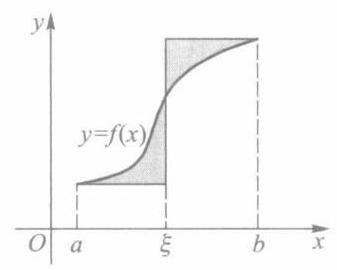
\includegraphics[width=.3\textwidth]{images/P064.jpg}
	\caption{图 $9-12$}
	\label{fig:P064}
\end{figure}

12. 设 \(f\) 为 \(\left\lbrack  {0,{2\pi }}\right\rbrack\) 上的单调递减函数. 证明: 对任何正整数 \(n\) ,恒有
\[
{\int }_{0}^{2\pi }f\left( x\right) \sin {nx}\mathrm{\;d}x \geq  0.
\]
13. 证明: 当 \(x > 0\) 时有不等式
\[
\left| {{\int }_{x}^{x + c}\sin {t}^{2}\mathrm{\;d}t}\right|  \leq  \frac{1}{x}\left( {c > 0}\right) .
\]
14. 证明: 若 \(f\) 在 \(\left\lbrack  {a,b}\right\rbrack\) 上可积, \(\varphi\) 在 \(\left\lbrack  {\alpha ,\beta }\right\rbrack\) 上严格单调且 \({\varphi }^{\prime }\) 在 \(\left\lbrack  {\alpha ,\beta }\right\rbrack\) 上可积, \(\varphi \left( \alpha \right)  = a,\varphi \left( \beta \right)  = b\) , 则有
\[
{\int }_{a}^{b}f\left( x\right) \mathrm{d}x = {\int }_{\alpha }^{\beta }f\left( {\varphi \left( t\right) }\right) {\varphi }^{\prime }\left( t\right) \mathrm{d}t.
\]
15. 若 \(f\) 在 \(\left\lbrack  {a,b}\right\rbrack\) 上连续可微,则存在 \(\left\lbrack  {a,b}\right\rbrack\) 上连续可微的增函数 \(g\) 和连续可微的减函数 \(h\) ,使得
\[
f\left( x\right)  = g\left( x\right)  + h\left( x\right) ,\;x \in  \left\lbrack  {a,b}\right\rbrack  .
\]
* 16. 证明: 若在 \(\left\lbrack  {a,b}\right\rbrack\) 上 \(f\) 为连续函数, \(g\) 为连续可微的单调函数,则存在 \(\xi  \in  \left\lbrack  {a,b}\right\rbrack\) ,使得
\[
{\int }_{a}^{b}f\left( x\right) g\left( x\right) \mathrm{d}x = g\left( a\right) {\int }_{a}^{\xi }f\left( x\right) \mathrm{d}x + g\left( b\right) {\int }_{\xi }^{b}f\left( x\right) \mathrm{d}x.
\]
(提示:与定理 9.11 及其推论相比较, 这里的条件要强得多, 因此可给出一个比较简单的、不同于定理 9.11 的证明.)

\section{* §6 可积性理论补叙}

\subsection{上和与下和的性质}

在 §3 第二段里,我们已经引入了上和 \(S\left( T\right)\) 和下和 \(s\left( T\right)\) 的概念. 即对于分割 \(T\) : \(a = {x}_{0} < {x}_{1} < \cdots  < {x}_{n} = b\) ,以及 \({\Delta }_{i} = \left\lbrack  {{x}_{i - 1},{x}_{i}}\right\rbrack  ,\Delta {x}_{i} = {x}_{i} - {x}_{i - 1}\) ,有
\[
S\left( T\right)  = \mathop{\sum }\limits_{{i = 1}}^{n}{M}_{i}\Delta {x}_{i},\;s\left( T\right)  = \mathop{\sum }\limits_{{i = 1}}^{n}{m}_{i}\Delta {x}_{i},
\]
其中 \({M}_{i} = \mathop{\sup }\limits_{{x \in  {\Delta }_{i}}}f\left( x\right) ,{m}_{i} = \mathop{\inf }\limits_{{x \in  {\Delta }_{i}}}f\left( x\right) ,i = 1,2,\cdots ,n\) . 由于假设 \(f\) 在 \(\left\lbrack  {a,b}\right\rbrack\) 上有界,因此上述 \({M}_{i},{m}_{i}\) 以及 \(f\) 在 \(\left\lbrack  {a,b}\right\rbrack\) 上的上、下确界 \(M\) 与 \(m\) 都存在,而且对于任何 \({\xi }_{i} \in  {\Delta }_{i}\) ,必有
\[
m\left( {b - a}\right)  \leq  s\left( T\right)  \leq  \mathop{\sum }\limits_{{i = 1}}^{n}f\left( {\xi }_{i}\right) \Delta {x}_{i} \leq  S\left( T\right)  \leq  M\left( {b - a}\right) . \tag{1}
\]
下面讨论上和与下和的性质. 借助这些性质, 便能由不等式 (1) 导出可积的充要条件.

性质 1 对同一个分割 \(T\) ,相对于任何点集 \(\left\{  {\xi }_{i}\right\}\) 而言,上和是所有积分和的上确界, 下和是所有积分和的下确界. 即
\[
S\left( T\right)  = \mathop{\sup }\limits_{\left| {\xi }_{i}\right| }\mathop{\sum }\limits_{{i = 1}}^{n}f\left( {\xi }_{i}\right) \Delta {x}_{i},\;s\left( T\right)  = \mathop{\inf }\limits_{\left| {\xi }_{i}\right| }\mathop{\sum }\limits_{{i = 1}}^{n}f\left( {\xi }_{i}\right) \Delta {x}_{i}.
\]
%证
\begin{proof}

\end{proof}
由不等式 (1) 知道,相对于任何点集 \(\left\{  {\xi }_{i}\right\}\) 而言,上和与下和分别是全体积分和的上界与下界. 现在进一步证明它们分别是全体积分和的最小上界与最大下界.

任给 \(\varepsilon  > 0\) ,在各个 \({\Delta }_{i}\) 上由于 \({M}_{i}\) 是 \(f\left( x\right)\) 的上确界,故可选取点 \({\xi }_{i} \in  {\Delta }_{i}\) ,使 \(f\left( {\xi }_{i}\right)  >\)  \({M}_{i} - \frac{\varepsilon }{b - a}\) . 于是有
\[
\mathop{\sum }\limits_{{i = 1}}^{n}f\left( {\xi }_{i}\right) \Delta {x}_{i} > \mathop{\sum }\limits_{{i = 1}}^{n}\left( {{M}_{i} - \frac{\varepsilon }{b - a}}\right) \Delta {x}_{i}
\]
\[
= \mathop{\sum }\limits_{{i = 1}}^{n}{M}_{i}\Delta {x}_{i} - \frac{\varepsilon }{b - a}\mathop{\sum }\limits_{{i = 1}}^{n}\Delta {x}_{i} = S\left( T\right)  - \varepsilon .
\]
这就证明了 \(S\left( T\right)\) 是全体积分和的上确界. 类似地可证 \(s\left( T\right)\) 是全体积分和的下确界. 性质 2 设 \({T}^{\prime }\) 为分割 \(T\) 添加 \(p\) 个新分点后所得到的分割,则有
\[
S\left( T\right)  \geq  S\left( {T}^{\prime }\right)  \geq  S\left( T\right)  - \left( {M - m}\right) p\parallel T\parallel , \tag{2}
\]
\[
s\left( T\right)  \leq  s\left( {T}^{\prime }\right)  \leq  s\left( T\right)  + \left( {M - m}\right) p\parallel T\parallel . \tag{3}
\]
这个性质指出:增加分点后,上和不增,下和不减.

%证
\begin{proof}

\end{proof}
这里证明不等式 (2) , 同理可证 (3).

将 \(p\) 个新分点同时添加到 \(T\) ,和逐个添加到 \(T\) ,都同样得到 \({T}^{\prime }\) ,所以我们先证 \(p = 1\) 的情形.

在 \(T\) 上添加 1 个新分点,它必落在 \(T\) 的某一小区间 \({\Delta }_{k}\) 上,而且将 \({\Delta }_{k}\) 分为两个小区间,记为 \({\Delta }_{k}^{\prime }\) 与 \({\Delta }_{k}^{\prime \prime }\) . 但 \(T\) 的其他小区间 \({\Delta }_{i}\left( {i \neq  k}\right)\) 仍旧是新分割 \({T}_{1}\) 所属的小区间. 因此, 比较 \(S\left( T\right)\) 与 \(S\left( {T}_{1}\right)\) 的各个被加项,它们之间的差别仅仅是 \(S\left( T\right)\) 中的 \({M}_{k}\Delta {x}_{k}\) 一项换成了 \(S\left( {T}_{1}\right)\) 中的 \({M}_{k}^{\prime }\Delta {x}_{k}^{\prime }\) 与 \({M}_{k}^{\prime \prime }\Delta {x}_{k}^{\prime \prime }\) 两项 (这里 \({M}_{k}^{\prime }\) 与 \({M}_{k}^{\prime \prime }\) 分别是 \(f\) 在 \({\Delta }_{k}^{\prime }\) 与 \({\Delta }_{k}^{\prime \prime }\) 上的上确界),所以
\[
S\left( T\right)  - S\left( {T}_{1}\right)  = {M}_{k}\Delta {x}_{k} - \left( {{M}_{k}^{\prime }\Delta {x}_{k}^{\prime } + {M}_{k}^{\prime \prime }\Delta {x}_{k}^{\prime \prime }}\right)
\]
\[
= {M}_{k}\left( {\Delta {x}_{k}^{\prime } + \Delta {x}_{k}^{\prime \prime }}\right)  - \left( {{M}_{k}^{\prime }\Delta {x}_{k}^{\prime } + {M}_{k}^{\prime \prime }\Delta {x}_{k}^{\prime \prime }}\right)
\]
\[
= \left( {{M}_{k} - {M}_{k}^{\prime }}\right) \Delta {x}_{k}^{\prime } + \left( {{M}_{k} - {M}_{k}^{\prime \prime }}\right) \Delta {x}_{k}^{\prime \prime }.
\]
由于
\[
m \leq  {M}_{k}^{\prime }\left( {\text{ 或 }{M}_{k}^{\prime \prime }}\right)  \leq  {M}_{k} \leq  M,
\]
故有
\[
0 \leq  S\left( T\right)  - S\left( {T}_{1}\right)  \leq  \left( {M - m}\right) \Delta {x}_{k}^{\prime } + \left( {M - m}\right) \Delta {x}_{k}^{\prime \prime }
\]
\[
= \left( {M - m}\right) \Delta {x}_{k} \leq  \left( {M - m}\right) \parallel T\parallel .
\]
这就证得 \(p = 1\) 时 (2) 式成立.

一般说来,对 \({T}_{i}\) 增加 1 个分点得到 \({T}_{i + 1}\) ,就有
\[
0 \leq  S\left( {T}_{i}\right)  - S\left( {T}_{i + 1}\right)  \leq  \left( {M - m}\right) \begin{Vmatrix}{T}_{i}\end{Vmatrix},i = 0,1,2,\cdots ,p - 1,
\]
(这里 \({T}_{0} = T,{T}_{p} = {T}^{\prime }\) ). 把这些不等式对 \(i\) 依次相加,得到
\[
0 \leq  S\left( T\right)  - S\left( {T}^{\prime }\right)  \leq  \left( {M - m}\right) \mathop{\sum }\limits_{{i = 0}}^{{p - 1}}\begin{Vmatrix}{T}_{i}\end{Vmatrix} \leq  \left( {M - m}\right) p\parallel T\parallel .
\]
这就证得 (2) 式成立.

性质 3 若 \({T}^{\prime }\) 与 \({T}^{\prime \prime }\) 为任意两个分割, \(T = {T}^{\prime } + {T}^{\prime \prime }\) 表示把 \({T}^{\prime }\) 与 \({T}^{\prime \prime }\) 的所有分点合并而得的分割 (注意:重复的分点只取一次), 则
\[
S\left( T\right)  \leq  S\left( {T}^{\prime }\right) ,\;s\left( T\right)  \geq  s\left( {T}^{\prime }\right) ,
\]
\[
S\left( T\right)  \leq  S\left( {T}^{\prime \prime }\right) ,\;s\left( T\right)  \geq  s\left( {T}^{\prime \prime }\right) .
\]
%证
\begin{proof}

\end{proof}
这是因为 \(T\) 既可看作 \({T}^{\prime }\) 添加新分点后得到的分割,也可看作 \({T}^{\prime \prime }\) 添加新分点后得到的分割, 所以由性质 2 立刻推知此性质成立.

性质 4 对任意两个分割 \({T}^{\prime }\) 与 \({T}^{\prime \prime }\) ,总有
\[
s\left( {T}^{\prime }\right)  \leq  S\left( {T}^{\prime \prime }\right) .
\]
%证
\begin{proof}

\end{proof}
令 \(T = {T}^{\prime } + {T}^{\prime \prime }\) . 由性质 1 与性质 3 便有
\[
s\left( {T}^{\prime }\right)  \leq  s\left( T\right)  \leq  S\left( T\right)  \leq  S\left( {T}^{\prime \prime }\right) .
\]
这个性质指出: 在对 \(\left\lbrack  {a,b}\right\rbrack\) 所作的任意两个分割中,一个分割的下和总不大于另一个分割的上和. 因此对所有分割来说, 所有下和有上界, 所有上和有下界, 从而分别存在上确界与下确界, 把它们记作
\[
S = \mathop{\inf }\limits_{T}S\left( T\right) ,\;s = \mathop{\sup }\limits_{T}s\left( T\right) .
\]
通常称 \(S\) 为 \(f\) 在 \(\left\lbrack  {a,b}\right\rbrack\) 上的上积分, \(s\) 为 \(f\) 在 \(\left\lbrack  {a,b}\right\rbrack\) 上的下积分.

性质 \({5m}\left( {b - a}\right)  \leq  s \leq  S \leq  M\left( {b - a}\right)\) .

这可由性质 4 直接推出.

性质 6 (达布定理) 上、下积分也是上和与下和在 \(\parallel T\parallel  \rightarrow  0\) 时的极限,即
\[
\mathop{\lim }\limits_{{\parallel T\parallel  \rightarrow  0}}S\left( T\right)  = S,\;\mathop{\lim }\limits_{{\parallel T\parallel  \rightarrow  0}}s\left( T\right)  = s.
\]
%证
\begin{proof}

\end{proof}
下面只证第一个极限.

任给 \(\varepsilon  > 0\) ,由 \(S\) 的定义,必存在某一分割 \({T}^{\prime }\) ,使得
\[
S\left( {T}^{\prime }\right)  < S + \frac{\varepsilon }{2}. \tag{4}
\]
设 \({T}^{\prime }\) 由 \(p\) 个分点所构成,对于任意另一个分割 \(T\) 来说, \(T + {T}^{\prime }\) 至多比 \(T\) 多 \(p\) 个分点,由性质 2 和性质 3 得到
\[
S\left( T\right)  - \left( {M - m}\right) p\parallel T\parallel  \leq  S\left( {T + {T}^{\prime }}\right)  \leq  S\left( {T}^{\prime }\right) .
\]
于是有
\[
S\left( T\right)  \leq  S\left( {T}^{\prime }\right)  + \left( {M - m}\right) p\parallel T\parallel .
\]
所以,只要 \(\parallel T\parallel  < \frac{\varepsilon }{2\left( {M - m}\right) p}\)\footnote{当 \(M = m\) 时 \(f\) 为常量函数,性质恒成立. 所以这里设 \(M > m\) .},就有 \(S\left( T\right)  \leq  S\left( {T}^{\prime }\right)  + \frac{\varepsilon }{2}\) . 联系 (4) 式,推得 \(S \leq  S\left( T\right)  < S +\)  \(\varepsilon\) . 这就证得
\[
\mathop{\lim }\limits_{{\parallel T\parallel  \rightarrow  0}}S\left( T\right)  = S.
\]
\subsection{可积的充要条件}

%定理 9.14
\begin{theorem}{}{the:}

\end{theorem}
(可积的第一充要条件)函数 \(f\) 在 \(\left\lbrack  {a,b}\right\rbrack\) 上可积的充要条件是: \(f\) 在 \(\left\lbrack  {a,b}\right\rbrack\) 上的上积分与下积分相等,即
\[
S = s.
\]
%证
\begin{proof}

\end{proof}
必要性 设 \(f\) 在 \(\left\lbrack  {a,b}\right\rbrack\) 上可积, \(J = {\int }_{a}^{b}f\left( x\right) \mathrm{d}x\) . 由定积分定义,任给 \(\varepsilon  > 0\) ,存在 \(\delta  > 0\) ,只要 \(\parallel T\parallel  < \delta\) ,就有
\[
\left| {\mathop{\sum }\limits_{{i = 1}}^{n}f\left( {\xi }_{i}\right) \Delta {x}_{i} - J}\right|  < \varepsilon .
\]
另一方面,由于 \(S\left( T\right)\) 与 \(s\left( T\right)\) 分别为积分和关于点集 \(\left\{  {\xi }_{i}\right\}\) 的上、下确界 (即性质 1),所以当 \(\parallel T\parallel  < \delta\) 时,又有
\[
\left| {S\left( T\right)  - J}\right|  \leq  \varepsilon ,\;\left| {s\left( T\right)  - J}\right|  \leq  \varepsilon .
\]
这说明当 \(\parallel T\parallel  \rightarrow  0\) 时 \(S\left( T\right)\) 与 \(s\left( T\right)\) 都以 \(J\) 为极限. 由达布定理 (即性质 6), \(S = s = J\) .

充分性 设 \(S = s = J\) . 由达布定理得
\[
\mathop{\lim }\limits_{{\parallel T\parallel  \rightarrow  0}}S\left( T\right)  = \mathop{\lim }\limits_{{\parallel T\parallel  \rightarrow  0}}s\left( T\right)  = J. \tag{5}
\]
借助不等式 (1),任给 \(\varepsilon  > 0\) ,存在 \(\delta  > 0\) ,当 \(\parallel T\parallel  < \delta\) 时,满足
\[
J - \varepsilon  < s\left( T\right)  \leq  \mathop{\sum }\limits_{{i = 1}}^{n}f\left( {\xi }_{i}\right) \Delta {x}_{i} \leq  S\left( T\right)  < J + \varepsilon .
\]
从而 \(f\) 在 \(\left\lbrack  {a,b}\right\rbrack\) 上可积,且 \({\int }_{a}^{b}f\left( x\right) \mathrm{d}x = J\) .

§3 例 1 提到的狄利克雷函数在 \(\left\lbrack  {0,1}\right\rbrack\) 上不可积,正是由于它的上积分 \(\left( {S = 1}\right)\) 与下积分 \(\left( {s = 0}\right)\) 不相等所致.



%定理 9.15
\begin{theorem}{}{the:}

\end{theorem}
 (可积的第二充要条件) 函数 \(f\) 在 \(\left\lbrack  {a,b}\right\rbrack\) 上可积的充要条件是: 任给 \(\varepsilon  > 0\) ,总存在某一分割 \(T\) ,使得
\[
S\left( T\right)  - s\left( T\right)  < \varepsilon \text{ ,即 }\mathop{\sum }\limits_{{i = 1}}^{n}{\omega }_{i}\Delta {x}_{i} < \varepsilon \text{ . }
\]
其中 \({\omega }_{i} = {M}_{i} - {m}_{i}\) ( \(f\) 在 \({\Delta }_{i}\) 上的振幅), \(i = 1,2,\cdots ,n\) .

此定理即为 §3 中未曾证明的可积准则.

%证
\begin{proof}

\end{proof}
必要性 设 \(f\) 在 \(\left\lbrack  {a,b}\right\rbrack\) 上可积,由定理 9.14 中的 (5) 式,有
\[
\mathop{\lim }\limits_{{\parallel T\parallel  \rightarrow  0}}\left\lbrack  {S\left( T\right)  - s\left( T\right) }\right\rbrack   = 0.
\]
于是,任给 \(\varepsilon  > 0\) ,只要 \(\parallel T\parallel\) 足够小,总存在分割 \(T\) ,使得
\[
S\left( T\right)  - s\left( T\right)  < \varepsilon .
\]
充分性 若定理条件得到满足, 则由
\[
s\left( T\right)  \leq  s \leq  S \leq  S\left( T\right)
\]
可推得
\[
0 \leq  S - s \leq  S\left( T\right)  - s\left( T\right)  < \varepsilon .
\]
由于 \(\varepsilon\) 的任意性,必有 \(S = s\) ,故由定理 9.14 证得 \(f\) 在 \(\left\lbrack  {a,b}\right\rbrack\) 上可积.

在 §3 证明可积函数类与 §4 讨论定积分的性质时,我们已经熟悉了可积第二充要条件的重要作用.

%定理 9.16
\begin{theorem}{}{the:}

\end{theorem}
(可积的第三充要条件)函数 \(f\) 在 \(\left\lbrack  {a,b}\right\rbrack\) 上可积的充要条件是:任给正数 \(\varepsilon ,\eta\) ,总存在某一分割 \(T\) ,使得属于 \(T\) 的所有小区间中,对应于振幅 \({\omega }_{{k}^{\prime }} \geq  \varepsilon\) 的那些小区间 \({\Delta }_{{k}^{\prime }}\) 的总长 \(\mathop{\sum }\limits_{{k}^{\prime }}\Delta {x}_{{k}^{\prime }} < \eta\) .

%证
\begin{proof}

\end{proof}
必要性 设 \(f\) 在 \(\left\lbrack  {a,b}\right\rbrack\) 上可积. 由定理 9.15,对于 \(\sigma  = {\varepsilon \eta } > 0\) ,存在某一分割 \(T\) , 使得 \(\mathop{\sum }\limits_{k}{\omega }_{k}\Delta {x}_{k} < \sigma\) . 于是便有
\[
\varepsilon \mathop{\sum }\limits_{{k}^{\prime }}\Delta {x}_{{k}^{\prime }} \leq  \mathop{\sum }\limits_{{k}^{\prime }}{\omega }_{{k}^{\prime }}\Delta {x}_{{k}^{\prime }} \leq  \mathop{\sum }\limits_{k}{\omega }_{k}\Delta {x}_{k} < {\varepsilon \eta },
\]
由此即得 \(\mathop{\sum }\limits_{{k}^{\prime }}\Delta {x}_{{k}^{\prime }} < \eta\) .

充分性 任给 \({\varepsilon }^{\prime } > 0\) ,取 \(\varepsilon  = \frac{{\varepsilon }^{\prime }}{2\left( {b - a}\right) } > 0,\eta  = \frac{{\varepsilon }^{\prime }}{2\left( {M - m}\right) } > 0\) . 由假设,存在某一分割 \(T\) ,使得 \({\omega }_{{k}^{\prime }} \geq  \varepsilon\) 的那些 \({\Delta }_{{k}^{\prime }}\) 的总长 \(\mathop{\sum }\limits_{{k}^{\prime }}\Delta {x}_{{k}^{\prime }} < \eta\) . 设 \(T\) 中其余满足 \({\omega }_{{k}^{\prime \prime }} < \varepsilon\) 的那些小区间为 \({\Delta }_{{k}^{\prime \prime }}\) , 则有
\[
\mathop{\sum }\limits_{k}{\omega }_{k}\Delta {x}_{k} = \mathop{\sum }\limits_{{k}^{\prime }}{\omega }_{{k}^{\prime }}\Delta {x}_{{k}^{\prime }} + \mathop{\sum }\limits_{{k}^{\prime \prime }}{\omega }_{{k}^{\prime \prime }}\Delta {x}_{{k}^{\prime \prime }}
\]
\[
< \left( {M - m}\right) \mathop{\sum }\limits_{{k}^{\prime }}\Delta {x}_{{k}^{\prime }} + \varepsilon \mathop{\sum }\limits_{{k}^{\prime \prime }}\Delta {x}_{{k}^{\prime \prime }}
\]
\[
\leq  \left( {M - m}\right) \eta  + \varepsilon \left( {b - a}\right)
\]
\[
= \frac{{\varepsilon }^{\prime }}{2} + \frac{{\varepsilon }^{\prime }}{2} = {\varepsilon }^{\prime }\text{ . }
\]
由定理 9.15 推知 \(f\) 在 \(\left\lbrack  {a,b}\right\rbrack\) 上可积.

%例 1
\begin{example}

\end{example}
用定理 9.16 证明黎曼函数在 \(\left\lbrack  {0,1}\right\rbrack\) 上可积,且定积分等于 0 .

%证
\begin{proof}

\end{proof}
在 §3 的例 3,我们曾用可积的第二充要条件证得黎曼函数在 \(\left\lbrack  {0,1}\right\rbrack\) 上可积. 现在改用第三充要条件来证明, 将更为简明.

已知黎曼函数为
\[
f\left( x\right)  = \left\{  \begin{array}{ll} \frac{1}{q}, & x = \frac{p}{q}\left( {p,q \in  {\mathbf{N}}_{ + },\frac{p}{q}\text{ 为既约真分数 }}\right) , \\  0, & x = 0,1\text{ 以及 }\left( {0,1}\right) \text{ 内的无理数. } \end{array}\right.
\]
任给 \(\varepsilon  > 0,\eta  > 0\) . 由于满足 \(\frac{1}{q} \geq  \varepsilon\) ,即 \(q \leq  \frac{1}{\varepsilon }\) 的有理点 \(\frac{p}{q}\) 只有有限个 (设为 \(K\) 个),因此含有这类点的小区间至多 \({2K}\) 个,在其上 \({\omega }_{{k}^{\prime }} \geq  \varepsilon\) . 当 \(\parallel T\parallel  < \frac{\eta }{2K}\) 时,就能保证这些小区间的总长满足
\[
\mathop{\sum }\limits_{{k}^{\prime }}\Delta {x}_{{k}^{\prime }} \leq  {2K}\parallel T\parallel  < \eta ,
\]
所以 \(f\) 在 \(\left\lbrack  {0,1}\right\rbrack\) 上可积.

因为 \({m}_{i} = \mathop{\inf }\limits_{{x \in  {\Delta }_{i}}}f\left( x\right)  = 0,i = 1,2,\cdots ,n\) ,所以 \(s\left( T\right)  = 0\) ,
\[
{\int }_{0}^{1}f\left( x\right) \mathrm{d}x = s = 0.
\]
%例 2
\begin{example}

\end{example}
证明: 若 \(f\) 在 \(\left\lbrack  {a,b}\right\rbrack\) 上连续, \(\varphi\) 在 \(\left\lbrack  {\alpha ,\beta }\right\rbrack\) 上可积, \(a \leq  \varphi \left( t\right)  \leq  b,t \in  \left\lbrack  {\alpha ,\beta }\right\rbrack\) ,则 \(f \circ  \varphi\) 在 \(\left\lbrack  {\alpha ,\beta }\right\rbrack\) 上可积.

%证
\begin{proof}

\end{proof}
任给 \(\varepsilon  > 0,\eta  > 0\) . 由于 \(f\) 在 \(\left\lbrack  {a,b}\right\rbrack\) 上一致连续,因此对上述 \(\eta\) ,存在 \(\delta  > 0\) ,当 \({x}^{\prime }\) , \({x}^{\prime \prime } \in  \left\lbrack  {a,b}\right\rbrack\) 且 \(\left| {{x}^{\prime } - {x}^{\prime \prime }}\right|  < \delta\) 时,
\[
\left| {f\left( {x}^{\prime }\right)  - f\left( {x}^{\prime \prime }\right) }\right|  < \eta .
\]
由假设 \(\varphi\) 在 \(\left\lbrack  {\alpha ,\beta }\right\rbrack\) 上可积,对上述正数 \(\delta\) 和 \(\varepsilon\) ,存在某一分割 \(T\) ,使得在 \(T\) 所属的小区间中, \({\omega }_{{k}^{\prime }}^{\varphi } \geq  \delta\) 的所有小区间 \({\Delta }_{{k}^{\prime }}\) 的总长 \(\mathop{\sum }\limits_{{k}^{\prime }}\Delta {t}_{{k}^{\prime }} < \varepsilon\) ; 而在其余小区间 \({\Delta }_{{k}^{\prime \prime }}\) 上 \({\omega }_{{k}^{\prime \prime }}^{\varphi } < \delta\) .

设 \(F\left( t\right)  = f\left( {\varphi \left( t\right) }\right) ,t \in  \left\lbrack  {\alpha ,\beta }\right\rbrack\) . 由以上可知: 在 \(T\) 中的小区间 \({\Delta }_{{k}^{\prime \prime }}\) 上, \({\omega }_{{k}^{\prime \prime }}^{F} < \eta\) ; 至多在所有 \({\Delta }_{{k}^{\prime }}\) 上 \({\omega }_{{k}^{\prime }}^{F} \geq  \eta\) ,而这些小区间的总长至多为 \(\mathop{\sum }\limits_{{k}^{\prime }}\Delta {t}_{{k}^{\prime }} < \varepsilon\) .

由可积的第三充要条件,证得复合函数 \(f \circ  \varphi\) 在 \(\left\lbrack  {\alpha ,\beta }\right\rbrack\) 上可积.

\subsection{习题 9.6}

1. 证明性质 2 中关于下和的不等式 (3).

2. 证明性质 6 中关于下和的极限式 \(\mathop{\lim }\limits_{{\parallel T\parallel  \rightarrow  0}}s\left( T\right)  = s\) .

3. 设
\[
f\left( x\right)  = \left\{  \begin{array}{ll} x, & x\text{ 为有理数, } \\  0, & x\text{ 为无理数. } \end{array}\right.
\]
试求 \(f\) 在 \(\left\lbrack  {0,1}\right\rbrack\) 上的上积分和下积分; 并由此判断 \(f\) 在 \(\left\lbrack  {0,1}\right\rbrack\) 上是否可积.

4. 设 \(f\) 在 \(\left\lbrack  {a,b}\right\rbrack\) 上可积,且 \(f\left( x\right)  \geq  0,x \in  \left\lbrack  {a,b}\right\rbrack\) . 试问 \(\sqrt{f}\) 在 \(\left\lbrack  {a,b}\right\rbrack\) 上是否可积? 为什么?

5. 证明: 定理 9.15 中的可积第二充要条件等价于 “任给 \(\varepsilon  > 0\) ,存在 \(\delta  > 0\) ,对一切满足

\(\parallel T\parallel  < \delta\) 的 \(T\) ,都有 \(\mathop{\sum }\limits_{T}{\omega }_{i}\Delta {x}_{i} = S\left( T\right)  - s\left( T\right)  < \varepsilon\) ".

6. 据理回答:

(1)何种函数具有“任意下和等于任意上和”的性质？

(2)何种连续函数具有“所有下和(或上和)都相等”的性质？

(3)对于可积函数,若“所有下和(或上和)都相等”,是否仍有(2)的结论？

7. 本题的最终目的是要证明: 若 \(f\) 在 \(\left\lbrack  {a,b}\right\rbrack\) 上可积,则 \(f\) 在 \(\left\lbrack  {a,b}\right\rbrack\) 上必定有无限多个处处稠密的连续点. 这可用区间套方法按以下顺序逐一证明:

(1) 若 \(T\) 是 \(\left\lbrack  {a,b}\right\rbrack\) 的一个分割,使得 \(S\left( T\right)  - s\left( T\right)  < b - a\) ,则在 \(T\) 中存在某个小区间 \({\Delta }_{i}\) ,使 \({\omega }_{i}^{f} < 1\) .

(2)存在区间 \({I}_{1} = \left\lbrack  {{a}_{1},{b}_{1}}\right\rbrack   \subset  \left( {a,b}\right)\) ,使得
\[
{\omega }^{f}\left( {I}_{1}\right)  = \mathop{\sup }\limits_{{x \in  {I}_{1}}}f\left( x\right)  - \mathop{\inf }\limits_{{x \in  {I}_{1}}}f\left( x\right)  < 1.
\]
(3)存在区间 \({I}_{2} = \left\lbrack  {{a}_{2},{b}_{2}}\right\rbrack   \subset  \left( {{a}_{1},{b}_{1}}\right)\) ,使得
\[
{\omega }^{f}\left( {I}_{2}\right)  = \mathop{\sup }\limits_{{x \in  {I}_{2}}}f\left( x\right)  - \mathop{\inf }\limits_{{x \in  {I}_{2}}}f\left( x\right)  < \frac{1}{2}.
\]
(4)继续以上方法,求出一区间序列 \({I}_{n} = \left\lbrack  {{a}_{n},{b}_{n}}\right\rbrack   \subset  \left( {{a}_{n - 1},{b}_{n - 1}}\right)\) ,使得
\[
{\omega }^{f}\left( {I}_{n}\right)  = \mathop{\sup }\limits_{{x \in  {I}_{n}}}f\left( x\right)  - \mathop{\inf }\limits_{{x \in  {I}_{n}}}f\left( x\right)  < \frac{1}{n}.
\]
说明 \(\left\{  {I}_{n}\right\}\) 为一区间套,从而存在 \({x}_{0} \in  {I}_{n},n = 1,2,\cdots\) ; 而且 \(f\) 在点 \({x}_{0}\) 连续.

(5)上面求得的 \(f\) 的连续点在 \(\left\lbrack  {a,b}\right\rbrack\) 上处处稠密.

\section{第九章总练习题}

1. 证明: 若 \(\varphi\) 在 \(\left\lbrack  {0,a}\right\rbrack\) 上连续, \(f\) 二阶可导,且 \({f}^{\prime \prime }\left( x\right)  \geq  0\) ,则有
\[
\frac{1}{a}{\int }_{0}^{a}f\left( {\varphi \left( t\right) }\right) \mathrm{d}t \geq  f\left( {\frac{1}{a}{\int }_{0}^{a}\varphi \left( t\right) \mathrm{d}t}\right) .
\]
2. 证明下列命题:

(1)若 \(f\) 在 \(\left\lbrack  {a,b}\right\rbrack\) 上连续增,
\[
F\left( x\right)  = \left\{  \begin{array}{ll} \frac{1}{x - a}{\int }_{a}^{x}f\left( t\right) \mathrm{d}t, & x \in  (a,b\rbrack , \\  f\left( a\right) , & x = a, \end{array}\right.
\]
则 \(F\) 为 \(\left\lbrack  {a,b}\right\rbrack\) 上的增函数.

(2)若 \(f\) 在 \(\lbrack 0, + \infty )\) 上连续,且 \(f\left( x\right)  > 0\) ,则
\[
\varphi \left( x\right)  = {\int }_{0}^{x}{tf}\left( t\right) \mathrm{d}t/{\int }_{0}^{x}f\left( t\right) \mathrm{d}t
\]
为 \(\left( {0, + \infty }\right)\) 上的严格增函数. 如果要使 \(\varphi\) 在 \(\lbrack 0, + \infty )\) 上为严格增,试问应补充定义 \(\varphi \left( 0\right)  =\) ?

3. 设 \(f\) 在 \(\lbrack 0, + \infty )\) 上连续,且 \(\mathop{\lim }\limits_{{x \rightarrow   + \infty }}f\left( x\right)  = A\) ,证明
\[
\mathop{\lim }\limits_{{x \rightarrow   + \infty }}\frac{1}{x}{\int }_{0}^{x}f\left( t\right) \mathrm{d}t = A.
\]
4. 设 \(f\) 是定义在 \(\left( {-\infty , + \infty }\right)\) 上的一个连续周期函数,周期为 \(p\) ,证明
\[
\mathop{\lim }\limits_{{x \rightarrow   + \infty }}\frac{1}{x}{\int }_{0}^{x}f\left( t\right) \mathrm{d}t = \frac{1}{p}{\int }_{0}^{p}f\left( t\right) \mathrm{d}t.
\]
5. 证明:连续的奇函数的一切原函数皆为偶函数；连续的偶函数的原函数中只有一个是奇函数.

6. 证明施瓦茨 (Schwarz) 不等式: 若 \(f\) 和 \(g\) 在 \(\left\lbrack  {a,b}\right\rbrack\) 上可积,则
\[
{\left( {\int }_{a}^{b}f\left( x\right) g\left( x\right) \mathrm{d}x\right) }^{2} \leq  {\int }_{a}^{b}{f}^{2}\left( x\right) \mathrm{d}x \cdot  {\int }_{a}^{b}{g}^{2}\left( x\right) \mathrm{d}x.
\]
7. 利用施瓦茨不等式证明:

(1)若 \(f\) 在 \(\left\lbrack  {a,b}\right\rbrack\) 上可积,则
\[
{\left( {\int }_{a}^{b}f\left( x\right) \mathrm{d}x\right) }^{2} \leq  \left( {b - a}\right) {\int }_{a}^{b}{f}^{2}\left( x\right) \mathrm{d}x;
\]
(2)若 \(f\) 在 \(\left\lbrack  {a,b}\right\rbrack\) 上可积,且 \(f\left( x\right)  \geq  m > 0\) ,则
\[
{\int }_{a}^{b}f\left( x\right) \mathrm{d}x \cdot  {\int }_{a}^{b}\frac{1}{f\left( x\right) }\mathrm{d}x \geq  {\left( b - a\right) }^{2};
\]
(3) 若 \(f,g\) 都在 \(\left\lbrack  {a,b}\right\rbrack\) 上可积,则有闵可夫斯基 (Minkowski) 不等式:
\[
{\left\lbrack  {\int }_{a}^{b}{\left( f\left( x\right)  + g\left( x\right) \right) }^{2}\mathrm{\;d}x\right\rbrack  }^{\frac{1}{2}} \leq  {\left\lbrack  {\int }_{a}^{b}{f}^{2}\left( x\right) \mathrm{d}x\right\rbrack  }^{\frac{1}{2}} + {\left\lbrack  {\int }_{a}^{b}{g}^{2}\left( x\right) \mathrm{d}x\right\rbrack  }^{\frac{1}{2}}.
\]

8. 证明: 若 \(f\) 在 \(\left\lbrack  {a,b}\right\rbrack\) 上连续,且 \(f\left( x\right)  > 0\) ,则
\[
\ln \left( {\frac{1}{b - a}{\int }_{a}^{b}f\left( x\right) \mathrm{d}x}\right)  \geq  \frac{1}{b - a}{\int }_{a}^{b}\ln f\left( x\right) \mathrm{d}x.
\]

9. 设 \(f\) 为 \(\left( {0, + \infty }\right)\) 上的连续减函数, \(f\left( x\right)  > 0\) ; 又设
\[
{a}_{n} = \mathop{\sum }\limits_{{k = 1}}^{n}f\left( k\right)  - {\int }_{1}^{n}f\left( x\right) \mathrm{d}x.
\]
证明 \(\left\{  {a}_{n}\right\}\) 为收敛数列.

10. 若 \(f\) 在 \(\left\lbrack  {0,a}\right\rbrack\) 上连续可微,且 \(f\left( 0\right)  = 0\) ,则
\[
{\int }_{0}^{a}\left| {f\left( x\right) {f}^{\prime }\left( x\right) }\right| \mathrm{d}x \leq  \frac{a}{2}{\int }_{0}^{a}{\left\lbrack  {f}^{\prime }\left( x\right) \right\rbrack  }^{2}\mathrm{\;d}x.
\]
11. 证明: 若 \(f\) 在 \(\left\lbrack  {a,b}\right\rbrack\) 上可积,且处处有 \(f\left( x\right)  > 0\) ,则 \({\int }_{a}^{b}f\left( x\right) \mathrm{d}x > 0\) .

(提示:由可积的第一充要条件进行反证;也可利用习题 9.6 第 7 题的结论.)

